\part{心电学中特殊检查、案例写作技巧及疑难解}

本篇内容侧重于心电学方面特殊检查的临床应用与评估、临床工作需要(规范心电图报告、撰写心电图案例论文)及复杂心律失常的分析诊断(实例精解)而编写,共4章。

\protect\hypertarget{text00056.html}{}{}

\protect\hypertarget{text00056.htmlux5cux23chapter56}{}{}

\chapter{心电学中特殊检查的临床应用及评估}

\protect\hypertarget{text00056.htmlux5cux23subid657}{}{}

\section{心率变异性分析}

心率变异性(HRV)即心搏间频率变异,反映了自主神经系统中交感与副交感神经对窦房结频率瞬时变化的调控,并受到大脑皮层活动、体液因素、压力反射和呼吸活动等因素的影响。通过HRV分析,能有效评估心脏植物神经功能状态,是判断多种心血管疾病预后及心源性猝死的一个相对独立性较强的指标。

\protect\hypertarget{text00056.htmlux5cux23subid658}{}{}

\subsection{HRV分析内容}

HRV分析包括时域分析和频域分析两方面的内容。

1.时域分析

时域分析以SDNN、SDNN\textsubscript{index}
、r-MSSD、PNN\textsubscript{50} 这4个指标最常用。

(1)平均R-R间期:测量某段时间内的窦性R-R间期的平均值。白天与夜间平均R-R间期互差<40ms为异常。

(2)总体标准差(SDNN):指24h内全部窦性R-R间期的标准差,正常值为100~150ms,<50ms为异常。

(3)均值标准差(SDANN):指24h内每5min节段窦性R-R间期平均值的标准差,正常值为80~140ms,<50ms为异常。

(4)标准差均值(SDNN\textsubscript{index}
):指24h内每5min节段窦性R-R间期平均值的标准差的平均值,正常值为40~80ms,<20ms为异常。

(5)差值的均方根(r-MSSD):指24h内相邻窦性R-R间期差值的均方根,正常值为15~45ms,<15ms为降低。

(6)相邻两个R-R间期差值>50ms的百分数(PNN\textsubscript{50}
):指24h内相邻两个窦性R-R间期差值>50ms的个数所占的百分率,正常值为1\%~12\%,<0.75\%为异常。

(7)Lorenz散点图:正常人均呈彗星状。

SDNN反映交感与副交感神经总的张力大小,SDANN、SDNN\textsubscript{index}
反映交感神经张力大小,与心率的缓慢变化成分相关,当交感神经张力增高时,其值降低;r-MSSD、PNN\textsubscript{50}
反映副交感神经张力大小,与心率的快速变化成分相关,当副交感神经张力降低时,其值降低。HRV随着年龄的增加而呈下降趋势。

2.频域分析

频域分析常用方法有回归法(AR法)和快速Fourier转换法(FFT法)两种。前者较为精确,且各频段曲线平滑,目测效果好,是目前推荐使用的方法;后者简单快速,但分辨率低。通常以频率(Hz)为横坐标,功率谱密度(PSD)为纵坐标的功率图谱,纵坐标单位为ms\textsuperscript{2}
/Hz。

频谱成分和频段划分:一般可分为5个频段。

(1)高频带(HF):0.15~0.4Hz,反映副交感神经的张力。

(2)中频带(MF):0.09~0.15Hz。

(3)低频带(LF):0.04~0.09Hz,反映交感和副交感神经的共同作用,但以前者为主。

(4)极低频带(VLF):0.0033~0.04Hz。

(5)超低频带(μLF):<0.0033Hz。

(6)总功率(TP):≤0.4Hz。

(7)LF/HF:反映交感-副交感神经的平衡状况。

功率谱密度(PSD)与LF、HF的归一化(norm)特点:前者较直观,后者能作个体化分析,能客观全面地反映交感、副交感神经活动的消长情况,其计算方法为:LF(HF)\textsubscript{norm}
=100×LF(HF)/(总功率-VLF),单位为nu。

短时程(5min)分析,反映患者固有的自主神经活动情况,采用TP、VLF、LF、HF、LF/HF、LF\textsubscript{norm}
及HF\textsubscript{norm}
;长时程(24h)分析反映总体综合情况,采用TP、ULF、VLF、LF、HF。

静卧5min记录的功率谱正常值范围为:

TP:3466±1018ms\textsuperscript{2} /Hz

LF:1170±416ms\textsuperscript{2} /Hz;LF\textsubscript{norm} :54±4nu

HF:975±203ms\textsuperscript{2} /Hz;HF:29±3nu

LF/HF:1.5~2.0

正常人交感、副交感神经支配心脏有着明显的昼夜变化规律:白天LF占优势,夜间HF占优势,LF在昼夜间基本保持不变,LF/HF在夜间的比值降低。

\protect\hypertarget{text00056.htmlux5cux23subid659}{}{}

\subsection{判断各种指标变化的临床意义}

SDANN、SDNN\textsubscript{index}
值降低,表明交感神经张力增高;r-MSSD、PNN\textsubscript{50}
值降低,表明副交感神经张力降低,但需结合年龄加以判断。

\protect\hypertarget{text00056.htmlux5cux23subid660}{}{}

\subsection{HRV临床应用评估}

自主神经系统与心源性猝死密切相关,心电稳定性有赖于交感、副交感神经和体液调节之间的平衡。若交感神经张力过度增高,则有利于致命性心律失常的发生;而副交感神经激活,则具有保护心脏和抗心室颤动作用。

(1)已有肯定应用价值的疾病:①急性心肌梗死:作为预测心肌梗死后死亡危险性的指标,SDNN<50ms者的死亡危险性比SDNN>100ms者高出5倍。②充血性心力衰竭:SDNN<50ms者,预测其死亡率的特异性>90\%,敏感性为75\%;LF<200ms\textsuperscript{2}
/Hz者,预测其死亡率的特异性>91\%,敏感性为75\%,HRV分析有望成为预测心力衰竭患者预后的独立指标。③糖尿病:HRV具有早期预报糖尿病并发神经病变的价值,为最准确、最敏感的指标。

(2)有研究前景的心血管疾病:有猝死倾向的二尖瓣脱垂症、心肌病、长Q-T间期综合征、高血压病、病毒性心肌炎、心脏移植及阵发性心动过速(如阵发性心房扑动、心房颤动、室上性心动过速)等。

(3)有研究前景的其他疾病:血管迷走性晕厥、体位性低血压、肝硬化、具有婴儿猝死综合征危险的婴儿和早产儿、药物对HRV的影响等。

\protect\hypertarget{text00056.htmlux5cux23subid661}{}{}

\section{窦性心律震荡现象}

1.基本概念

室性早搏对随后的窦性频率的影响有两种情况:①窦性频率先加速,后减速,形成双相涨落式变化,这种特征性的变化称为窦性心律震荡现象,见于正常人及心肌梗死后猝死的低危患者;②窦性频率改变不明显或消失,见于心肌梗死后猝死的高危患者。

2.检测方法

(1)震荡初始(TO):用室性早搏后的前2个窦性R-R间期的均值(用A表示)减去偶联间期前的2个窦性R-R间期的均值(用B表示),两者之差除以后者,即TO=(A-B)/B。

(2)震荡斜率(TS):是定量分析室性早搏后是否存在窦性频率减速现象。先测算早搏后的前20个窦性R-R间期值,并以R-R间期值为纵坐标,以R-R间期的序号为横坐标,绘制R-R间期值的分布图,再用任意连续5个序号的R-R间期值计算并作出回归线,其中正向的最大斜率为TS的结果。TS值以每个R-R间期的ms变化值表示,当TS>2.5ms/R-R间期时,表明存在减速现象;当TS<2.5ms/R-R间期时,表明不存在减速现象。

3.发生机制

(1)室性早搏的直接作用:早搏引起动脉内血压下降,代偿间歇后第1个窦性搏动的动脉血压将上升,这些变化将影响窦房结血液供应及对窦房结机械性牵张作用,影响窦房结自律性。

(2)室性早搏的反射作用:通过压力感受器发生的压力反射是出现窦性心律震荡现象的最主要机制。

4.应用与评价

TO和TS指标对猝死高危患者预测作用稳定而可靠。

(1)预测急性心肌梗死后猝死危险性:TO、TS均异常时,是猝死最敏感的预测指标,其阳性预测精确度达32\%,同时阴性预测精确度达90\%。

(2)预测慢性心力衰竭患者的预后和猝死的危险性。

\protect\hypertarget{text00056.htmlux5cux23subid662}{}{}

\section{心室晚电位和心房晚电位}

心室晚电位(VLP)和心房晚电位(ALP)可用信号平均心电图(SAECG)来描记。

\protect\hypertarget{text00056.htmlux5cux23subid663}{}{}

\subsection{心室晚电位(VLP)}

1.概述

VLP是心室舒张末期出现高频、低振幅的碎裂心电活动,表现为QRS波群终末端、ST段上微弱碎裂的心电活动信号。该信号来自心肌缓慢传导的区域,表明心室内存在潜在的折返环,易形成快速性室性心律失常,对心肌梗死病人的预后预测、冠心病、心力衰竭患者猝死危险性预测有着重要意义。检测方法有时域分析(TDA)、频域分析(STM)及时频三维图,以时域分析最常用。

2.VLP的识别

(1)确定VLP起点:QRS终末部低于40μV处作为VLP的起点。

(2)确定VLP终点:把基础噪声(ST段后半部<1μV)作为参照点,当低振幅高频波大于基础噪声3倍时,作为VLP终点。

(3)确定VLP时间:VLP起点至终点的距离便是VLP时间,至少为10ms。

(4)测定总QRS波群时间(QRS-D):在经过滤波的综合导联叠加心电图上,从QRS起点至VLP终点的时距。

(5)测定RMS\textsubscript{40}
:测定经过滤波的综合导联叠加心电图的QRS波群最后40ms内的振幅,如≤25μV,表明有VLP存在。

(6)测定总QRS波群终末向量振幅低于40μV者(LAS)持续时间:如≥40ms,表明有VLP存在。

3.VLP阳性的判断标准

除外束支阻滞,高频截止频率为25Hz的条件下,TDA分析符合下列标准中两项者可确定VLP阳性:①QRS-D≥120ms;②LAS\textsubscript{40}
≥40ms;③RMS\textsubscript{40}
≤25μV。高频截止频率为40Hz的条件下,其阳性标准为:①QRS-D≥114ms;②LAS\textsubscript{40}
≥38ms;③RMS\textsubscript{40}
≤20μV。STM分析在X、Y、Z轴任一导联上的正常因子(NF)<30\%,即可确定为VLP阳性。

4.临床应用

(1)预测心肌梗死后发生恶性心律失常:VLP的TDA法能有效预测心律失常事件,具有高度特异性、中度敏感性,阳性预测精确度为30\%,阴性预测精确度>95\%,可作为危险度的分层筛选方法之一;STM法预测心律失常事件特异性90\%、敏感性75\%,但其诊断标准有待完善。

(2)预测各类心肌病患者发生恶性心律失常。

\protect\hypertarget{text00056.htmlux5cux23subid664}{}{}

\subsection{心房晚电位(ALP)}

ALP阳性对预测心房颤动的发生有一定价值,其阳性标准为:Ad(P波时间)≥145ms,LP\textsubscript{30}
(终末30ms)<3μV。

\protect\hypertarget{text00056.htmlux5cux23subid665}{}{}

\section{T波电交替及T波变异性分析}

\protect\hypertarget{text00056.htmlux5cux23subid666}{}{}

\subsection{T波电交替}

1.基本概念

T波电交替是指起源于同一节律点的搏动在同一导联中,T波的形态、振幅、极性出现逐搏交替性变化,其振幅互差≥0.1mV,并排除呼吸、体位、伪差及心包积液等心外因素的影响,可同时伴有QRS波群、ST段等波段的电交替。

2.分类

有宏观T波电交替及微观T波电交替两类。前者指肉眼可以观察到,而后者则需借助特殊信号处理技术才能发现的微伏级T波电交替。

3.微伏级T波电交替检测方法

有频谱分析法、复合解调分析法及相关分析法,目前应用最多的是频谱分析法。适用于已知或疑有发生恶性室性心律失常及猝死危险性的患者,如各种器质性心脏病尤其是心肌梗死患者、不明原因晕厥、各类心肌病、长Q-T间期综合征患者等。

\protect\hypertarget{text00056.htmlux5cux23subid667}{}{}

\subsection{T波变异性分析}

1.基本概念

T波变异性是指T波形态、振幅随每次心搏发生周期性改变,但缺乏T波电交替时2:1典型变化规律。

2.检测计算方法

(1)依赖于Q-T间期的T波变异性检测:将Q-T间期变异性与R-R间期变异性(即心率变异性)的比值定义为Q-T变异指数(QTVI)。QTVI反映的是T波时间的变异情况,当其≥0.1时,发生室性心律失常猝死的概率增高。

(2)不依赖于Q-T间期的T波变异性检测:①成分波分析法:利用同步12导联心电图比较两个连续心搏在不同频率带的子波变异性,分析T波时间变异性与振幅变异性两个参数,若这两个心搏的两个参数有差异,则为阳性。②相关性分析法:为T波信号的时域分析方法,用复极相关指数反映复极变异性,即将心率基本相同的连续T波与一个T波模板分别进行比较,若一致,则无T波变异;若不一致,则存在T波变异。

\protect\hypertarget{text00056.htmlux5cux23subid668}{}{}

\section{直立倾斜试验}

1.试验方法

(1)普通直立倾斜试验:①安静、平卧10~20min;②倾斜角度60°~80°;③倾斜时间30min。

(2)分级直立倾斜试验:①倾斜角度加大至80°;②倾斜时间延长至45min。

(3)药物激发倾斜试验:①异丙基肾上腺素1μg/(kg·min),共10min;2μg/(kg·min),共10min;3μg/(kg·min),共10min。②其他药物,如硝酸甘油、三磷酸腺苷、肾上腺素等。

2.结果判定

根据临床症状及心率、血压的变化判断结果。在倾斜试验中,若患者出现以下改变之一者,可判定为阳性:①发生晕厥或接近晕厥症状;②收缩压下降至80mmHg以下和(或)舒张压下降至50mmHg以下或平均动脉压下降25\%;③心率减慢:包括窦性心动过缓(<50次/min)、窦性停搏代之以房室交接性逸搏心律、一过性二度及以上的房室传导阻滞或长达3.0s以上的心脏停搏。阳性结果对血管性晕厥具有诊断意义。敏感性为32\%~85\%,特异性为90\%,重复性可达65\%~85\%。

3.适应证

(1)器质性心脏病同时伴有不能解释的晕厥;

(2)无器质性心脏病而有反复晕厥出现;

(3)老年人不能解释的晕厥;

(4)评估药物疗效。

4.禁忌证

有严重左心室流出道狭窄、重度二尖瓣狭窄、重度冠状动脉狭窄、重度脑动脉狭窄者应属于禁忌证。

5.反映方式

(1)血管抑制型:以血压下降为主。

(2)心脏抑制型:以心率明显减慢或停搏为主。

(3)混合型:血压下降同时伴有明显的心率减慢。

6.血管迷走神经性晕厥特点

(1)年轻人多见,以10~50岁为主。

(2)常无器质性心脏病。

(3)有明显诱因。

(4)有先兆症状。

(5)直立倾斜试验阳性。

\protect\hypertarget{text00056.htmlux5cux23subid669}{}{}

\section{心脏变时性功能不全}

1.基本概念

(1)心率储备:机体极量运动时所能达到的最高心率与静息时最低心率之间的差值,称为心率储备。

(2)心脏变时性功能:正常窦房结在神经、体液等因素调节下,根据机体不同状况,在较大范围内改变心率的快慢以满足机体供血、代谢的需要,这种功能称为心脏变时性功能。

(3)心脏变时性功能不全:窦房结对运动或代谢等病理生理变化丧失了应有的正常心率反应,即心率增快未达到一定程度,称为心脏变时性功能不全。

(4)心脏变时性功能过度:指运动时出现心率增快的反应高于预测最大值,超过了机体代谢需要。

2.检测方法

最重要检测方法是平板运动试验,以次极量运动为主和逐步加大运动负荷的方案,除能作出定性判断外,还能进行定量分析;其次是动态心电图检查及校正的窦房结恢复时间。

3.心脏变时性功能分类

(1)心脏变时性功能正常(图\ref{fig47-1})。

\begin{figure}[!htbp]
 \centering
 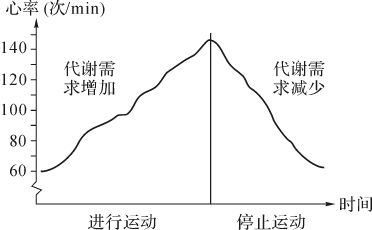
\includegraphics[width=2.51042in,height=1.55208in]{./images/Image00738.jpg}
 \captionsetup{justification=centering}
 \caption{变时性功能正常者运动时心率变化曲线示意图}
 \label{fig47-1}
  \end{figure} 

(2)完全性变时性功能不全:运动时窦性频率不增加或最大心率明显低于预测值(图\ref{fig47-2})。

\begin{figure}[!htbp]
 \centering
 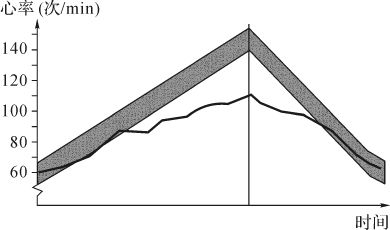
\includegraphics[width=2.63542in,height=1.55208in]{./images/Image00739.jpg}
 \captionsetup{justification=centering}
 \caption{完全性变时性功能不全患者运动时心率变化曲线示意图(极量运动时,最大心率明显低于预测值,且运动时初始阶段及恢复阶段心率反应显著降低)}
 \label{fig47-2}
  \end{figure} 

(3)与运动有关的变时性功能不全:①运动早期变时性功能不全型:指运动开始阶段心率增长明显低于正常,而运动后半段心率增长较快,可达到预测最大心率值,运动停止后心率下降与正常相似(图\ref{fig47-3});②运动后期变时性功能不全型:指运动开始阶段,心率随着运动量增加而加快,进一步增加运动量时,心率不再继续增加;③停止运动后心率速降型:指运动时变时性功能正常,但停止运动后,心率骤然下降,并在较短时间内降回运动前水平,与迷走神经张力过高有关,易发生迷走神经性晕厥(图\ref{fig47-4})。

\begin{figure}[!htbp]
 \centering
 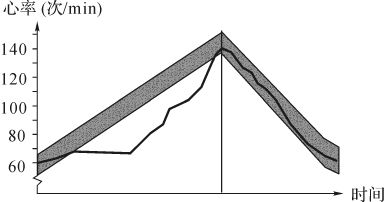
\includegraphics[width=2.59375in,height=1.36458in]{./images/Image00740.jpg}
 \captionsetup{justification=centering}
 \caption{运动早期变时性功能不全型心率变化曲线示意图(极量运动,最大心率与预测值相近,但运动时初始阶段心率反应显著降低或延迟)}
 \label{fig47-3}
  \end{figure} 

\begin{figure}[!htbp]
 \centering
 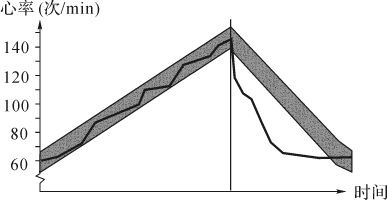
\includegraphics[width=2.61458in,height=1.34375in]{./images/Image00741.jpg}
 \captionsetup{justification=centering}
 \caption{停止运动后心率速降型心率变化曲线示意图(运动时初始反应及最大心率与预测值相近,但在运动结束后,心率迅速下降,并可出现长R-R间歇)}
 \label{fig47-4}
  \end{figure} 

(4)变异型变时性功能不全:在运动中,心率的变化与运动量的大小无关,难以预测(图\ref{fig47-5})。

\begin{figure}[!htbp]
 \centering
 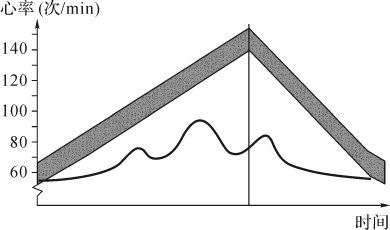
\includegraphics[width=2.63542in,height=1.55208in]{./images/Image00742.jpg}
 \captionsetup{justification=centering}
 \caption{变异型变时性功能不全心率变化曲线示意图(运动时心率波动很大且无规律,最大心率明显低于预测值,约占所有变时性功能不全75\%)}
 \label{fig47-5}
  \end{figure} 

4.评定标准

(1)最快心率达到最大预测心率百分比:最大预测心率计算方法为220-年龄(岁)。当最快心率达到最大预测心率的90\%以上时,心脏变时性功能正常;当最快心率达到最大预测心率的75\%~89\%时,为轻度的心脏变时性功能不全;当最快心率低于最大预测心率的75\%时,为明显的心脏变时性功能不全;当最快心率超过最大预测心率时,为心脏变时性功能过度。

(2)变时性指数:变时性指数=心率储备/代谢储备。

心率储备=(运动后心率-静息心率)/(最大预测心率-静息心率)

代谢储备=(运动后代谢值-1)/(极量运动的代谢值-1)

变时性指数正常值为0.8~1.3,当变时性指数<0.8时,为心脏变时性功能不全;当变时性指数>1.3时,为心脏变时性功能过度。

5.变时性功能不全的临床意义

许多器质性心脏病可导致心脏变时性功能不全,如冠心病、病窦综合征、严重的左心功能不全等。

(1)冠心病:运动试验中无ST段压低而有变时性功能不全者,经冠状动脉造影,72\%患者有明显的冠状动脉病变;运动试验中有ST段压低伴变时性功能不全者,冠状动脉三支病变的发生率高于仅有ST段压低者。提示运动试验中出现变时性功能不全是诊断冠心病一个独立而敏感的阳性指标,也是冠心病事件(如心绞痛、心肌梗死、猝死)发生风险及预后判断指标之一。

(2)心力衰竭:左心功能不全患者,变时性功能不全的特征是静息心率增加而最大心率减少,导致变时性指数降低。

(3)病窦综合征:变时性功能不全者多见,约占54\%,表现为静息心率下降,运动时心率轻微增加,运动耐量差,运动停止后心率恢复呈速降型。

(4)抗心律失常药物:是引发变时性功能不全的重要因素或直接原因,尤其是β受体阻滞剂,且与剂量呈正相关关系。

(5)指导选择合适的起搏器:变时性功能不全患者,选择具有频率应答功能起搏器,可使部分患者变时性功能不全情况得到逆转。

(6)变时性功能过度诱发心动过速性心肌病:心脏变时性功能过度的患者常有不适宜性窦性心动过速,长期心动过速可引发心功能减退,出现心动过速性心肌病,产生严重的临床后果。

\protect\hypertarget{text00056.htmlux5cux23subid670}{}{}

\section{动态心电图的临床应用}

\protect\hypertarget{text00056.htmlux5cux23subid671}{}{}

\subsection{概述}

动态心电图又称为活动心电图、长时间记录心电图,简称DCG。1957年由美国物理学家Holter博士首创,1961年应用于临床。随着电子技术的迅速发展,仪器不断更新,由原来双通道发展到三通道、十二通道,由磁带记录发展到闪光卡、SD片记录,体积更加细巧,分析软件更加先进、快捷,并拓展了检测功能,如心率变异性分析、心率震荡、T波电交替检测等,使其临床应用范围更加广泛,已成为心血管疾病检测不可缺少的重要的无创检查项目之一。

\protect\hypertarget{text00056.htmlux5cux23subid672}{}{}

\subsection{动态心电图的优、缺点}

1.优点

(1)DCG是在日常活动状态下作长时间记录,不受活动、体位限制,全面地反映患者在一天完整生物周期内的心电变化。

(2)DCG可连续记录24~72h,一份24h记录可获得约10万次心搏,能捕捉一过性和间歇性心电变化,特别是心律失常、心肌缺血,尤其是无症状性心肌缺血。

(3)DCG可确定心电异常与各种活动及症状之间的关系。

(4)DCG可明确心律失常分布规律,是白天多发还是夜间多发、是活动时多发还是静息时多发。

(5)DCG为无创性检查,安全、方便、可重复检查。

2.缺点

(1)DCG诊断属回顾性诊断,对严重心律失常有时会痛失抢救机会,我们曾遇5例Ron-T室性早搏诱发极速型室性心动过速、心室颤动而猝死。

(2)费用相对较高。

(3)活动量太大时,伪差波较多,影响分析的准确性。

(4)双通道、三通道记录,会漏诊高侧壁、下壁心肌缺血。

(5)DCG为模拟波形,其形态与常规心电图相应导联有一定的变异性。

\protect\hypertarget{text00056.htmlux5cux23subid673}{}{}

\subsection{动态心电图机的装置及电极安置的部位}

1.动态心电图机的装置

由随身佩带的小型记录盒及回放分析系统两部分组成。2009年9月,浙江大学生物医学工程与仪器科学学院及杭州百慧医疗设备有限公司联合成功研制了具有全自主知识产权、国际先进水平的CardioTrak动态心电分析系统。其中CT-08动态心电记录盒小巧轻便,重量仅为80g;高清晰度液晶显示,能实时观察各导联心电信号;1节7号碱性电池可持续记录96h;有单独的起搏信号检测通道,方便起搏心电图的分析和诊断。CardioTrak分析软件由浙江大学医学院附属邵逸夫医院心电图室全体同仁参与改进。该软件具有自动分析速度快(24h三通道的心电数据全部分析仅需10s)、结果准确(经MIT-BIH心律失常数据库检测,QRS波群和心律失常事件检出率高达99.6\%和92.7\%以上)及操作方便等特点;该软件还具有精确而强大的模板分类、灵活的导联选择、简洁高效的操作模式、准确的伪差识别、丰富的配置选项以及完整的智能分析工具(包括ST段分析、HRV时域与频域分析、T波电交替分析、窦性心律震荡分析等功能)等多项特点。该仪器已具备了与国外著名医疗仪器公司(如GE、Burdick等)同类产品竞争的实力,相信一定为国人带来福音(图\ref{fig47-6}、图\ref{fig47-7})。

\begin{figure}[!htbp]
 \centering
 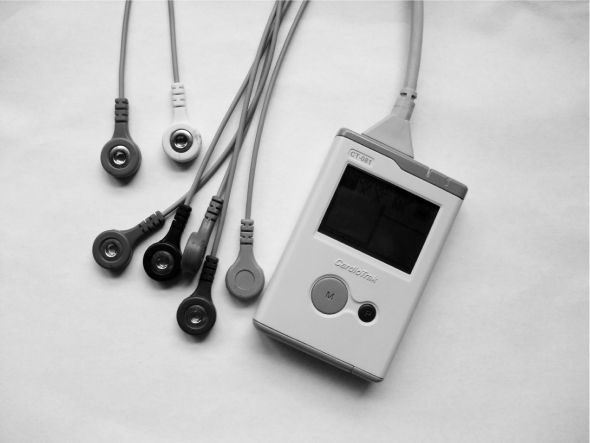
\includegraphics[width=3.98958in,height=2.98958in]{./images/Image00743.jpg}
 \captionsetup{justification=centering}
 \caption{CT-08动态心电记录盒}
 \label{fig47-6}
  \end{figure} 

\begin{figure}[!htbp]
 \centering
 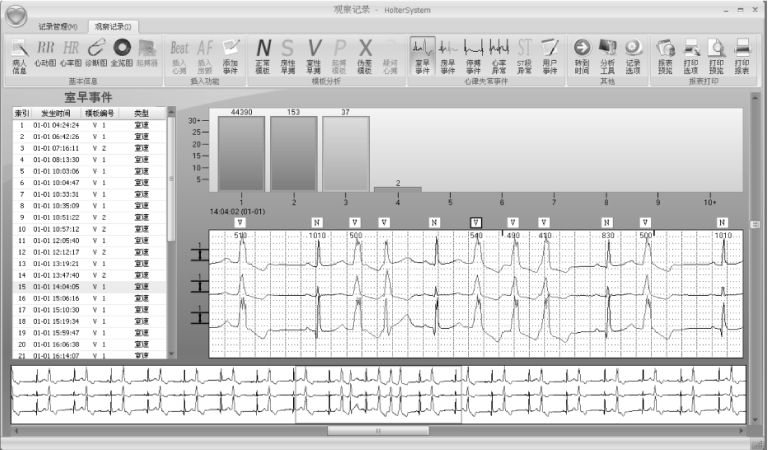
\includegraphics[width=5.1875in,height=3.04167in]{./images/Image00744.jpg}
 \captionsetup{justification=centering}
 \caption{快速、准确、简洁的CardioTrak动态心电分析软件}
 \label{fig47-7}
  \end{figure} 

2.电极安置的部位

(1)MV\textsubscript{1}
导联:正极贴在胸骨右缘第4肋间(V\textsubscript{1}
),负极贴在第2肋胸骨柄左侧。

(2)MV\textsubscript{5}
导联:正极贴在左侧腋前线第5肋(V\textsubscript{5}
),负极贴在第2肋胸骨柄右侧。

(3)MaVF导联:正极贴在左侧腋前线第9~10肋,负极贴在第2肋胸骨中线。本人不认可该导联是模拟aVF导联,从波形特点看,类似MV\textsubscript{5}
导联波形(图\ref{fig47-8}A)。我们一般将该导联正极贴在左侧锁骨中线第5肋(V\textsubscript{4}
)位置(图\ref{fig47-8}B),与MV\textsubscript{5} 导联一起监测前壁心肌供血情况。

\begin{figure}[!htbp]
 \centering
 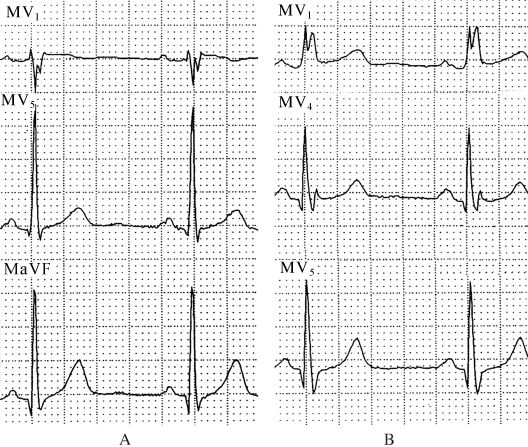
\includegraphics[width=3.5625in,height=3.02083in]{./images/Image00745.jpg}
 \captionsetup{justification=centering}
 \caption{图A按照“MaVF导联”位置贴的电极,MaVF导联波形与MV\textsubscript{5}}
 \label{fig47-8}
  \end{figure} 
导联波形类似;图B“MaVF导联”按照MV\textsubscript{4}
导联位置贴的电极,其波形与MV\textsubscript{5} 导联波形类似

(4)无关电极或地线:一般贴在右侧腋前线第5肋。

MV\textsubscript{1}
导联P波清晰,有利于心律失常分析和判断,MV\textsubscript{4}
、MV\textsubscript{5} 导联适合于观察前壁心肌缺血。

\protect\hypertarget{text00056.htmlux5cux23subid674}{}{}

\subsection{动态心电图的临床应用}

(一)健康人群的体检

1.心率

正常人心率平均在59~89次/min,活动时最高可达180次/min,夜间睡眠时最低不少于40次/min。

2.正常人可见的心律失常

(1)窦性心律不齐。

(2)室上性心律失常:约50\%~75\%可检出房性早搏,若早搏数>100次/24h或>总心率数的1/1000次,则属异常;约25\%~59\%可检出短阵性房性心动过速。

(3)室性心律失常:约50\%可检出室性早搏,早搏数量标准同上。

(4)房室传导阻滞:夜间可出现一度~二度Ⅰ型房室传导阻滞,可能与迷走神经张力增高有关。

(5)ST-T改变:心率增快时,以R波为主导联其ST段可压低,T波可低平;心率减慢时,则其ST段可呈凹面向上型抬高,T波可高耸。

(二)心律失常的监测

DCG对心律失常的观察和诊断具有独到之处,能明确持续时间、数量、起始、终止以及与日常生活或症状之间的关系,能完整地观察其演变过程和规律,尤其是夜间入睡时出现的各种心律失常、一过性或间歇性心律失常。

(三)心肌病的监测

心肌病DCG主要表现为心肌劳损及复杂性心律失常两种,有助于阐明心肌病患者某些症状的性质,尤其是晕厥症状发作是流出道狭窄所致,还是室性心动过速、心室扑动、心室颤动或停搏所致,有助于心肌病患者预后的判断及药物疗效的观察。

(四)心源性猝死机制的分析

心源性猝死多发生在器质性心脏病,尤其是急性心肌梗死后、重度心力衰竭、心肌病及原发性离子通道疾病等,如DCG检出复杂的室性早搏、室性心动过速、窦性停搏、二度Ⅱ型以上的房室传导阻滞,则猝死的危险性大大增高。有文献报道61例佩带DCG期间发生猝死,其中57例死于室性心动过速、心室颤动,4例死于缓慢性心律失常引起心脏停搏。我们曾遇5例Ron-T室性早搏诱发极速型室性心动过速、心室颤动而猝死(其中1例突发急性心肌梗死)。

(五)识别与心脏病有关的症状

临床上常遇及一些如胸闷、胸痛、气急、心悸、黑矇、晕厥或停跳感等症状,其原因是多方面的,如DCG发现一过性、间歇性心律失常或ST-T改变等与症状出现时间相吻合,则有助于症状的解释,作出合理判断与治疗。病人所述的停跳感可以是窦性停搏、窦房传导阻滞或房室传导阻滞所致,也可以是早搏、窦性心律不齐等。值得一提的是,有些严重心律失常甚至急性心肌梗死病人可无任何症状。晕厥的原因较多,有心源性和非心源性两大类。若DCG检测到长R-R间歇(>3.5~5.0s)、心室率极快的心动过速及恶性室性心律失常,则有利于心源性晕厥的诊断。DCG对识别心绞痛、变异性心绞痛、夜间阵发性呼吸困难是比较理想的诊断方法。

(六)人工起搏器的监测

(1)DCG能如实地反映起搏器的功能状态,如起搏功能、感知功能、频率、脉冲幅度、宽度、波形特点等,对改进起搏器性能提供依据。

(2)DCG对起搏器安装早期,能监测其起搏功能、感知功能是否正常,借以了解心内膜电极有无移位、漂移等。

(3)对后期能监测起搏器电池耗损程度、有无起搏与感知功能异常。

(七)病窦综合征的监测

可提高病窦综合征的诊断率,筛选需要安装人工起搏器患者。

(八)肺心病的监测

(九)呼吸睡眠暂停综合征的监测

(十)心力衰竭时心律失常的监测

(十一)冠心病的监护

心肌缺血检测方法有常规心电图、运动试验、DCG监测、ECT、心脏超声波、冠状动脉造影等。DCG能检测到冠心病患者在各种诱因下如劳累、情绪波动、紧张、用力排便、烟酒刺激等所出现的一过性ST-T改变。DCG可揭示无痛性、隐匿性缺血性ST-T改变,因其无症状,极易被疏忽。

DCG还可检出有猝死倾向的高危病例。引起猝死的重要原因是严重的心律失常,DCG则可发现短暂而严重的心律失常如室性心动过速等,以便及时治疗。多数学者认为冠心病患者出现复杂性室性早搏可增加心源性猝死的发生率,且这些患者大多有多支血管病变及心功能降低。

(十二)研究和评价药物的效果

DCG检查不仅有助于选择有效的抗心律失常药和评定其疗效,还可观察有无致心律失常性副作用。

(1)抗心律失常药物治疗有效标志:①早搏数量减少>55\%;②复杂性室性早搏数量减少>70\%;③短阵性室性心动过速发作减少>90\%;④持续性室性心动过速消失。

(2)抗心律失常药物致心律失常作用的诊断标准:请见第四十六章第二节抗心律失常药物致心律失常作用。

(十三)HRV分析、窦性心律震荡现象、T波变异性分析

请见本章第一、二、四节相关内容。

\protect\hypertarget{text00056.htmlux5cux23subid675}{}{}

\section{平板运动试验}

请见第四十二章第一节冠心病。

\protect\hypertarget{text00057.html}{}{}

\protect\hypertarget{text00057.htmlux5cux23chapter57}{}{}

\chapter{规范心电图诊断报告}

\protect\hypertarget{text00057.htmlux5cux23subid676}{}{}

\section{如何出具心电图诊断报告}

目前各地尚未有一个统一的、规范化的心电图诊断报告,有时将非特异性ST-T改变诊断为心肌缺血、心肌劳损或慢性冠状动脉供血不足等,易引发医源性或“心电图性”心脏病。现结合我们多年临床心电图工作经验,初步拟定出具心电图诊断报告的基本原则和格式,以期抛砖引玉、取得共识,完善心电图诊断报告之目的。

\protect\hypertarget{text00057.htmlux5cux23subid677}{}{}

\subsection{出具心电图诊断报告的基本原则}

临床各种疾病的诊断,大多包括病因诊断、病理解剖诊断、病理生理诊断及主要疾病诊断、次要疾病诊断等。临床诊断疾病的思维方法也适用于心电图诊断,心电图诊断也需要“由此及彼、由表及里、去伪存真”及尽量用“一元论”、最常见疾患来诊断的逻辑思维方法。

(1)一份心电图诊断报告,先要确定基本节律及其频率的快慢:根据有无P波及P波的极性、F波、f波等来确定基本节律是窦性、房性还是房室交接性、室性,再根据频率的快慢及节律规则与否,确定有无频率过速、过缓、不齐、停搏、外出阻滞等。

(2)一般情况下,诊断顺序可按心脏除极、复极的顺序,如P波、P-R间期、QRS波群、J点(J波)、ST段、Q-T间期、T波、U波的顺序进行诊断,如遇危急而严重的心电图改变需要急诊处理的,如急性心肌梗死、持续性快速性心律失常、较长时间的心室停搏等特殊情况,则应将此类诊断提前到第2条诊断。

(3)先描述所见的心电现象,后描述该心电现象所提示的临床意义或发生机制或需进一步做哪些检查以明确诊断。如“肺型P波,提示不完全性右心房内传导阻滞,建议做胸片或心脏超声心动图检查,以诊除右心房肥大”、“多源性室性早搏,其中一源为室性并行心律”。

(4)诊断心律失常时,必须写出异位起搏点的部位、发放冲动的强度(如正常频率、加速的、过速的、过缓的、早搏、逸搏、停搏等)、冲动在各个部位的传导情况及其伴随现象等,必须先写原发性心律失常,后写继发性及伴随心律失常,如“三度房室传导阻滞、缓慢的房室交接性逸搏心律”等。

(5)诊断起搏器功能异常时,尽量避免“起搏器故障”、“起搏器失灵”等不良性诊断用语,以避免医患之间造成不必要的纠纷。

(6)尽量用“一元论”及最常见的心电图诊断来解释所见的各种心电现象。

(7)诊断时,可根据明确的程度,用直接诊断法、提示诊断法、可疑或待排诊断法、符合诊断法等,如“左心室肥大伴劳损”、“提示左心室肥大”、“左心室肥大可疑(或待排)”、“符合低钾血症的心电图改变”等。

(8)诊断时,必须密切结合临床及电生理检查,符合目前公认的各种理论和心电现象,各个诊断之间不能自相矛盾。

(9)最好能结合前、后心电图片子或随访,特别是对宽QRS心动过速的诊断、疑有急性心肌梗死或左束支阻滞、预激综合征合并急性心肌梗死尤为重要。

\protect\hypertarget{text00057.htmlux5cux23subid678}{}{}

\subsection{规范心电图诊断报告格式}

心电图诊断的第1条必须是主导节律,如窦性心律、心房颤动、心房扑动、房性心律、房室交接性心律等,第2条诊断为所见的异常心电现象及其诊断和(或)机制。以下罗列常见的、但各地不很统一的报告格式,供参考。

(1)窦性心律、心电图正常范围。有以下心电图表现之一者可考虑心电图正常范围:①P波电轴左偏;②单纯的QRS电轴偏移在-30°~+120°之间;③单纯的逆钟向、顺钟向转位;④室上嵴型QRS波群,即V\textsubscript{1}
导联呈rSr′型,r>r′;⑤QRS终末波较宽钝,但QRS波群时间≤0.10s;⑥Ⅱ导联T波直立,振幅>$\frac{1}{10}$
R,aVF导联T波低平或平坦,Ⅲ导联T波倒置;⑦青少年出现T\textsubscript{v\textsubscript{1}}
、\textsubscript{v\textsubscript{2}}
>T\textsubscript{v\textsubscript{5}}
、\textsubscript{v\textsubscript{6}}
>$\frac{1}{10}$
R;⑧童稚型(幼年型)T波改变;⑨以R波为主导联ST段呈缺血型压低≤0.05mV(aVL、Ⅲ导联可压低0.1mV)或呈近水平型压低<0.08mV或呈上斜型压低<0.1mV;⑩心率较慢时以R波为主导联J点抬高,ST段呈凹面向上型抬高<0.1mV;\textcircled{11}
婴幼儿出现右心室电势占优势,即出现电轴右偏、V\textsubscript{1}
导联以R波为主。

(2)窦性心律、心电图大致正常。该诊断比较模糊,易引发患者不满或纠纷,尽量少用此诊断。有正常范围心电图改变≥2条者,可考虑用心电图大致正常的诊断。

(3)窦性心律、肺型P波(或二尖瓣型P波),提示右(左)心房肥大或右(左)心房负荷过重或不完全性右(左)心房内传导阻滞,请结合临床。

(4)窦性心律、间歇性肺型P波及二尖瓣型P波,为间歇性不完全性右心房、左心房内传导阻滞。

(5)窦性心律、V\textsubscript{1}
Ptf值增大,提示左心房负荷过重,请结合临床。

(6)窦性心律、S\textsubscript{Ⅰ} S\textsubscript{Ⅱ} S\textsubscript{Ⅲ}
综合征(假性电轴左偏、顺钟向转位),右心室肥大待排,请结合临床。(7)窦性心律、左心室高电压。年轻人、胸壁菲薄者、体力劳动者出现肢体导联和(或)胸前导联QRS波群电压增高者,可能是一种正常现象。

(8)窦性心律、左心室高电压,提示左心室肥大,请结合临床。临床上有引起左心室肥大的病理因素,如高血压病等,肢体导联和(或)胸前导联QRS波群电压显著增高,但无ST-T改变者。

(9)窦性心律、左心室高电压、ST-T改变,提示左心室肥大伴劳损,请结合临床。

(10)窦性心律、心电轴左偏-31°~-44°,若QRS波形符合左前分支阻滞图形特征,可提示左前分支阻滞;若不符合左前分支阻滞图形特征,仅诊断为心电轴左偏。

(11)窦性心律、下壁异常Q波可疑。Ⅱ导联QRS波呈R型或qR型,Ⅲ导联呈QS或QR型,aVF导联呈QR型,Q波>14R,但时间<0.03s。该心电图表现需结合临床病史或以往心电图片子,若曾有下壁心肌梗死病史,则可诊断为下壁异常Q波,陈旧性心肌梗死所致。

(12)窦性心律、前壁异常Q波伴ST段损伤型改变,符合急性心肌梗死的心电图改变(临床上已明确诊断为心肌梗死)或提示急性心肌梗死,请进一步做心肌酶谱检测(会诊单上仅写明胸痛)或亚急性心肌梗死(会诊单上已写明心肌梗死1周后)或提示陈旧性心肌梗死伴室壁瘤形成,请进一步做心脏超声心动图检查(心肌梗死3个月至半年后)。

(13)窦性心律、隐匿性不完全性右束支阻滞。V\textsubscript{1}
导联QRS波呈rSr′s′型或呈rS型,S波错折,其他导联QRS终末波较宽钝,时限≤0.11s,加做V\textsubscript{3}
R、V\textsubscript{4} R或V\textsubscript{1}
导联上一肋、下一肋出现rRr′型,则诊断为隐匿性不完全性右束支阻滞。

(14)窦性心律、P-R间期缩短(≤0.10s)。若患者有反复发作心动过速史,则诊断为L-G-L综合征;若无明显心动过速史,则诊断为L-G-L综合征待排或P-R间期缩短,请结合临床。

(15)窦性心律、前间壁ST段呈穹窿型或马鞍型改变。若仅有心电图改变,而无家族史或室性心动过速史、晕厥史,则提示为Brugada征或Brugada波或Brugada综合征样心电图改变;若有家族史或反复发作室性心动过速史、晕厥史,则提示为Brugada综合征。

(16)窦性心律、前侧壁或(和)下壁ST段抬高。若心率较慢时出现ST段呈凹面向上型抬高,同时伴J点抬高、T波高耸,活动后心率增快时J点、ST段抬高程度减轻或恢复正常,则诊断为早复极综合征;若心率较快时出现ST段呈凹面向上型抬高伴T波低平,临床上疑为心包炎时,则诊断为符合急性心包炎的心电图改变;若ST段呈上斜型抬高伴T波高耸,需结合临床提示为超急性期心肌梗死或变异型心绞痛,建议进一步检测心肌酶谱;若ST段呈弓背向上型或单向曲线型或巨“R”型抬高时,则提示急性心肌损伤或急性心肌梗死,建议进一步检测心肌酶谱、心电图动态观察。

(17)窦性心律、前侧壁或(和)下壁ST段压低。一般情况下,诊断为ST段改变即可。若ST段呈缺血型压低≥0.2~0.3mV,同时伴有胸痛,则诊断为ST段改变,符合心绞痛的心电图改变或急性心内膜下心肌梗死待排,建议进一步检测心肌酶谱;若ST段呈鱼钩样压低,患者正在服用洋地黄,则诊断为ST段改变,提示洋地黄作用。

(18)窦性心律、前侧壁或(和)下壁ST段呈水平型延长(ST段时间>0.16s)。若患者为冠心病,则提示心内膜下心肌缺血;若患者为慢性肾功能不全,建议血钙检测以诊除低钙血症。

(19)窦性心律、前侧壁或(和)下壁T波高耸(T波振幅>1.0mV)。若患者伴有胸痛发作,则诊断为超急性期心肌梗死或变异型心绞痛待排,建议进一步检测心肌酶谱;若患者有急性肾功能衰竭,则提示为高钾血症的心电图改变,建议血钾检测;若患者身体素质很好,心率较慢,则提示为早复极综合征所致;若患者有二尖瓣关闭不全或主动脉瓣关闭不全,则提示为左心室舒张期负荷过重所致;若脑血管意外、颅脑损伤后出现T波高耸,则提示为脑源性T波改变。

(20)窦性心律、前侧壁或(和)下壁T波低平或倒置。一般情况下,诊断为T波改变即可。若T波呈“冠状T波”,则诊断为“冠状T波”改变,请结合临床;若T波呈巨大倒置伴基底部宽阔、顶部切迹,则诊断为“尼加拉瓜瀑布样T波”改变,请结合临床;若T波两肢呈不对称性倒置、基底部较窄,同时伴ST段压低,则提示心肌劳损;若T波倒置与心室起搏器有关,则提示为心室电张力调整性T波改变(属功能性改变)。

(21)窦性心律、U波改变。若U波振幅增高,同时伴ST段压低、T波低平、Q-T间期延长,则结合临床诊断为符合低钾血症心电图改变、药物性(主要是抗心律失常药物)或脑源性(脑血管意外、颅脑损伤)心电图改变;若U波倒置或负正双相,则结合临床诊断为心肌劳损或供血不足或老年性U波改变。

(22)有关房性早搏二、三联律的诊断问题:因诊断某某心律时,必须要求该起搏点至少连续发放3次冲动(包括外出阻滞的冲动在内)。房性早搏二联律时,窦性激动与房性早搏呈交替性控制心房,且后者往往使前者节律重整,窦性冲动没有连续发放3次冲动,故不能诊断为窦性心律,只能诊断为窦性搏动、频发房性早搏二联律,若房性早搏呈双源性、多源性或双形性、多形性或为并行心律或呈阻滞型、干扰性P′-R间期延长及心室内差异性传导时,诊断时均应全部写上,如窦性搏动、频发多源性房性早搏呈二联律,有时伴干扰性P′-R间期延长及心室内差异性传导,其中一源为房性并行心律,这样就将房性早搏的发生程度、发生机制、传导情况全部诊断上。写上干扰性P′-R间期延长而有别于房性早搏通过房室结慢径路下传,写上心室内差异性传导排除了该宽大畸形QRS-T波群是室性早搏的可能。同样道理,房性早搏三联律时,也不能诊断为窦性心律,只能诊断为成对窦性搏动。

(23)有关短阵性(或短串性)室性异位心律的诊断问题:室性异位兴奋性增高引起的心律失常,由于异位灶自律性强度的改变,其连续发放3次以上的冲动有时以早搏、加速的室性逸搏或室性逸搏形式出现,此时的心电图既不能诊断为室性心动过速,又不能诊断为室性逸搏心律,那怎么办呢?可诊断为由室性早搏、加速的室性逸搏、室性逸搏组成的短阵性室性异位心律。

(24)有关起搏器的诊断问题:①先确定心脏本身的基本节律,后确定起搏器的类型(是单腔、双腔还是三腔起搏器);②确定是什么原因需要安装起搏器(是显著的窦性心动过缓、高度窦房传导阻滞、窦性停搏还是三度房室传导阻滞、双束支阻滞、三分支阻滞);③确定起搏器的起搏功能、感知功能及有无起搏源性心律失常;④确定有无其他的心电图异常改变。诊断时应注意完整性,不要遗漏。若遇及起搏器功能异常或可能异常时,需及时与临床医生沟通,共同确认诊断报告,尽量避免使用“起搏器故障”的诊断报告。这里着重讨论起搏器功能异常时的相关诊断:①起搏器故障的诊断:只有同时出现起搏功能不良和感知功能异常或出现频率奔放现象时,方可诊断为“起搏器故障”。②起搏功能异常的诊断:凡是落在心房、心室不应期以外的起搏信号不能夺获心房、心室产生相应的P′波或R′波时,则诊断为“起搏器起搏功能不良”;若起搏器发放频率异常,在排除起搏器频率奔放前提下,可诊断为“起搏器频率异常,请结合临床”。③感知功能异常的诊断:凡起搏器不能感知自身心电信号,仍按原有的起搏频率发放脉冲,与自身节律发生竞争现象,则诊断为“起搏器感知功能不良或低下,请调整感知灵敏度”;若起搏器感知到肌电信号、T波、交叉感知、电磁信号、静电磁场等引起起搏周期延长、不规则或暂停起搏,则诊断为“起搏器感知功能过强,请调整感知灵敏度”。④起搏源性心律失常的诊断:若有起搏器介导性心动过速、起搏器频率奔放现象、室房逆传诱发房性心律失常、反复心搏二联律或反复性心动过速、起搏-夺获二联律、Ron-T诱发的室性心动过速、心室颤动等心律失常时,则直接诊断之。⑤起搏器功能正常的诊断:凡是起搏器起搏功能良好、发放频率正常及感知功能良好时,可诊断为“未见起搏器功能异常”,亦尽量避免使用“起搏器功能正常”的诊断。

\protect\hypertarget{text00057.htmlux5cux23subid679}{}{}

\section{建立临床心电图诊断库}

随着网络化心电图机的发展及患者数量激增,有必要建立简捷而规范的临床心电图诊断库,借以提高工作效率。现结合我们多年工作经验,初步拟定临床心电图诊断报告格式,建立常用的诊断库。

\protect\hypertarget{text00057.htmlux5cux23subid680}{}{}

\subsection{正常心电图及其变异}

(1)窦性心律、心电图正常。

(2)窦性心律、心电图正常范围。

(3)窦性心律、心电图大致正常。

\protect\hypertarget{text00057.htmlux5cux23subid681}{}{}

\subsection{P波变异}

(1)电轴左偏型P波。

(2)二尖瓣型P波,提示左心房负荷过重、左心房肥大(或扩大)或不完全性左心房内传导阻滞。

(3)肺型P波,提示右心房负荷过重、右心房肥大(或扩大)或不完全性右心房内传导阻滞。

(4)先心型P波,提示右心房负荷过重或右心房肥大(或扩大)。

(5)巨大型P波,提示双心房负荷过重、双心房肥大(或扩大)、右心房肥大合并不完全性左心房内传导阻滞或左心房肥大合并不完全性右心房内传导阻滞、不完全性双心房内传导阻滞。

(6)间歇性二尖瓣型P波、肺型P波,为间歇性或频率依赖性不完全性左心房内、右心房内传导阻滞。

(7)右位心型P波。

(8)单纯性P波电交替现象。

(9)房间隔阻滞型P波,为完全性房间隔内传导阻滞伴左心房逆行传导,提示巴氏束传导阻滞。

(10)V\textsubscript{1} Ptf值增大,提示左心房负荷过重或肥大(或扩大)。

\protect\hypertarget{text00057.htmlux5cux23subid682}{}{}

\subsection{QRS波群变异}

(1)低电压、低电压倾向。

(2)左心室高电压。

(3)左心室高电压,提示左心室肥大。

(4)左心室高电压伴ST-T改变,提示左心室肥大伴劳损。

(5)左心室劳损。

(6)右心室电势占优势。

(7)右心室肥大。

(8)右心室肥大伴劳损。

(9)双心室肥大待排、提示双心室肥大、双心室肥大伴劳损。

(10)电轴左偏(中度、重度)。

(11)电轴右偏(中度、重度)。

(12)假性电轴左偏(S\textsubscript{Ⅰ} S\textsubscript{Ⅱ}
S\textsubscript{Ⅲ} 综合征)。

(13)QRS波幅电交替或电阶梯现象。

\protect\hypertarget{text00057.htmlux5cux23subid683}{}{}

\subsection{ST段变异}

(1)非特异性ST段改变。

(2)ST段呈损伤型(弓背向上型、单向曲线型、水平型、墓碑型、巨R型)抬高,提示或符合急性心肌梗死、变异型心绞痛、急性心包炎或左心室室壁瘤的心电图改变。

(3)ST段呈缺血型(水平型、下斜型)压低,提示左心室劳损、心肌供血不足或符合心绞痛发作的心电图改变。

(4)右胸导联ST段呈穹隆型或马鞍型抬高,符合Brugada波(征)或提示Brugada综合征。

(5)ST段呈水平型延长,提示心内膜下心肌缺血或符合低钙血症的心电图改变。

(6)ST段缩短。

(7)ST段呈电交替现象。

\protect\hypertarget{text00057.htmlux5cux23subid684}{}{}

\subsection{T波变异}

(1)非特异性T波改变。

(2)劳损型T波改变,提示左心室劳损或符合心尖肥厚型心肌病、肥厚性梗阻型心肌病的心电图改变。

(3)冠状T波改变,提示心肌供血不足或劳损。

(4)巨倒型T波改变。

(5)帐篷状T波改变,符合高钾血症的心电图改变。

(6)高耸型T波改变:提示左心室舒张期负荷过重、迷走神经张力过高、变异型心绞痛、超急性期心肌梗死、脑血管意外等。

(7)电张力调整性T波改变(属功能性改变,为正常的电生理现象)。

(8)T\textsubscript{v\textsubscript{1}}
、\textsubscript{v\textsubscript{2}}
>T\textsubscript{v\textsubscript{5}}
、\textsubscript{v\textsubscript{6}} 综合征。

(9)功能性T波改变(孤立性负T综合征、童稚型T波改变、“两点半”综合征、体位性T波改变、过度通气性T波改变、饱餐后T波改变)。

(10)早搏后T波改变。

(11)与心动周期长短有关的T波改变。

(12)T波电交替现象。

\protect\hypertarget{text00057.htmlux5cux23subid685}{}{}

\subsection{U波变异}

(1)U波增高,提示或符合低钾血症、脑血管意外或抗心律失常药物所致。

(2)U波极性改变(倒置、负正或正负双相),提示左心室早期劳损、心肌缺血或老年性改变。

(3)U波电交替现象。

(4)U波消失。

\protect\hypertarget{text00057.htmlux5cux23subid686}{}{}

\subsection{Q-T间期变异}

(1)Q-T间期延长,提示原发性或继发性长Q-T间期综合征。

(2)Q-T间期缩短,提示原发性或继发性短Q-T间期综合征。

\protect\hypertarget{text00057.htmlux5cux23subid687}{}{}

\subsection{J波、Epsilon波、Brugada波}

(1)异常J波:有原发性、继发性及缺血性J波之分。

(2)可见Epsilon波,符合右心室发育不良性心肌病的心电图改变。

(3)Brugada波:提示Brugada综合征、Brugada波,请结合临床判断。

\protect\hypertarget{text00057.htmlux5cux23subid688}{}{}

\subsection{异常Q波及其范畴}

(1)异常Q波。

(2)前间壁或前壁r波振幅递增不良。

(3)前间壁或前壁r波振幅逆递增。

\protect\hypertarget{text00057.htmlux5cux23subid689}{}{}

\subsection{心肌梗死}

(1)超急性期心肌梗死:有高侧壁、下壁、前间壁、前壁、前侧壁、后壁、广泛前壁之分。

(2)急性期心肌梗死:有高侧壁、下壁、前间壁、前壁、前侧壁、后壁、广泛前壁之分。

(3)亚急性期心肌梗死:有高侧壁、下壁、前间壁、前壁、前侧壁、后壁、广泛前壁之分。

(4)陈旧性期心肌梗死:有高侧壁、下壁、前间壁、前壁、前侧壁、后壁、广泛前壁之分。

(5)特殊类型心肌梗死:有急性心房梗死、急性右心室心肌梗死、急性心内膜下心肌梗死、急性非穿透性心肌梗死、再发性心肌梗死之分。

\protect\hypertarget{text00057.htmlux5cux23subid690}{}{}

\subsection{窦性心律失常}

(1)窦性心律不齐:有呼吸性、非呼吸性、室相性之分。

(2)窦性心动过速:有一般性、不适当性、体位性之分。

(3)窦性心动过缓:有一般性过缓(心率46~59次/min)、显著性过缓(≤45次/min)之分。

(4)窦性停搏。

(5)窦房传导阻滞:有2:1阻滞、二度Ⅰ型、二度Ⅱ型、高度、几乎完全性及三度传导阻滞之分。

(6)病窦综合征:有原发性、继发性、特发性之分,可分为Ⅰ、Ⅱ、Ⅲ、Ⅳ型。

(7)双结病。

(8)双结病伴短暂性全心停搏或心室停搏(R-R间期≥3.5~5.0s)。

(9)慢-快综合征:即心动过缓-心动过速综合征。

(10)快-慢综合征:即心动过速-心动过缓综合征。

(11)窦房结内游走性心律。

\protect\hypertarget{text00057.htmlux5cux23subid691}{}{}

\subsection{早搏}

(1)窦性早搏:有折返型、自律性增高型、并行心律型及触发型之分。

(2)窦房交接性早搏。

(3)房性早搏:有折返型(双形性、多形性)、自律性增高型(双源性、多源性)、并行心律型之分,可伴有各种房室干扰现象(阻滞型、干扰性P′-R间期延长、房室结内隐匿性传导、心室内差异性传导)。

(4)房室交接性早搏:有折返型、自律性增高型、并行心律型之分,可伴有心室内差异性传导。

(5)室性早搏:有折返型(双形性、多形性)、自律性增高型(双源性、多源性)、并行心律型之分。

(6)房室旁道性早搏:多为自律性增高型、并行心律型。

\protect\hypertarget{text00057.htmlux5cux23subid692}{}{}

\subsection{逸搏和逸搏心律}

(1)窦性逸搏。

(2)房性逸搏和逸搏心律:有过缓型、正常频率型、加速型之分,可呈双源性或多源性,可伴有起步现象或冷却现象。

(3)房室交接性逸搏和逸搏心律:有过缓型、正常频率型、加速型之分,可伴有非时相性心室内差异性传导,可呈双源性或多源性,可伴有起步现象或冷却现象。

(4)室性逸搏和逸搏心律:有过缓型、正常频率型、加速型之分,可呈双源性或多源性,可伴有起步现象或冷却现象。

(5)房室旁道性逸搏和逸搏心律。

\protect\hypertarget{text00057.htmlux5cux23subid693}{}{}

\subsection{心房及心室内差异性传导}

(1)心房内差异性传导:有时相性、非时相性之分。

(2)心室内差异性传导:有时相性、非时相性之分。

\protect\hypertarget{text00057.htmlux5cux23subid694}{}{}

\subsection{扑动和颤动}

(1)心房扑动(Ⅰ型、Ⅱ型)伴正常心室率、缓慢的心室率、快速的心室率。

(2)心房颤动(阵发性、持续性、永久性)伴正常心室率、缓慢的心室率、快速的心室率。

(3)尖端扭转型心房扑动伴正常心室率、缓慢的心室率、快速的心室率。

(4)不纯性心房扑动伴正常心室率、缓慢的心室率、快速的心室率。

(5)不纯性心房颤动伴正常心室率、缓慢的心室率、快速的心室率。

(6)心房颤动-心房扑动伴正常心室率、缓慢的心室率、快速的心室率。

(7)心室扑动。

(8)心室颤动:有原发性、继发性、特发性之分。

\protect\hypertarget{text00057.htmlux5cux23subid695}{}{}

\subsection{传导阻滞}

(1)窦房传导阻滞:有2:1阻滞、二度Ⅰ型、二度Ⅱ型、高度、几乎完全性及三度传导阻滞之分。

(2)心房内传导阻滞:①不完全性左心房、右心房内传导阻滞,可表现为间歇性、频率依赖性、固定性阻滞;②完全性心房内传导阻滞,即心房分离。

(3)房室传导阻滞:一度、二度(有二度Ⅰ型、Ⅱ型、高度、几乎完全性及2:1阻滞之分)、三度传导阻滞,可伴有房室超常期传导。

(4)房室交接区双层阻滞。

(5)房室交接区三层阻滞。

(6)左束支及其分支阻滞:①左束支阻滞:有不完全性、完全性及文氏型阻滞之分,可表现为间歇性、频率依赖性、固定性阻滞;②左前分支阻滞;③左后分支阻滞;④左中隔支阻滞:有Ⅰ型、Ⅱ型之分。

(7)右束支阻滞:有不完全性、完全性及文氏型阻滞之分,可表现为间歇性、频率依赖性、固定性阻滞。

(8)双束支阻滞:间歇性左右束支阻滞、完全性左束支阻滞伴房室传导阻滞型、部分完全性右束支阻滞伴房室传导阻滞型。

(9)双分支阻滞:左前分支阻滞合并左中隔支阻滞、左后分支阻滞合并左中隔支阻滞、间歇性左前及左后分支阻滞。

(10)双支阻滞:右束支阻滞合并左前分支阻滞、右束支阻滞合并左后分支阻滞、右束支阻滞合并左中隔支阻滞。

(11)三支阻滞:①右束支阻滞、左前分支阻滞合并房室传导阻滞型;②右束支阻滞、左后分支阻滞合并房室传导阻滞型;③间歇性出现右束支、左前、左后分支阻滞;④右束支阻滞、左前分支阻滞合并左中隔支阻滞;⑤右束支阻滞、左后分支阻滞合并左中隔支阻滞。

(12)不定型心室内传导阻滞。

(13)房室旁道性阻滞:有一度、二度Ⅰ型、二度Ⅱ型、高度阻滞,可表现为频率依赖性、间歇性阻滞。

\protect\hypertarget{text00057.htmlux5cux23subid696}{}{}

\subsection{双径路、多径路传导及反复搏动}

(1)窦房交接区内双径路传导。

(2)心房折返径路内双径路传导。

(3)房室交接区内双径路传导:有顺向型、逆向型、双向型双径路传导之分。

(4)房室交接区内三径路传导:有顺向型、逆向型、双向型三径路传导之分。

(5)心室折返径路内双径路传导。

(6)窦性回波。

(7)房性反复搏动。

(8)房室交接性反复搏动。

(9)室性反复搏动。

\protect\hypertarget{text00057.htmlux5cux23subid697}{}{}

\subsection{宽QRS心动过速}

(1)室性心动过速:按发作特点可分为短阵性、阵发性、非阵发性室性心动过速;按QRS波形特点可分为单形性、多形性、双向性、尖端扭转型性、分支性室性心动过速;按发生机制可分为折返型、自律性增高型、并行心律型、触发型室性心动过速。

(2)室上性心动过速伴心室内差异性传导、束支阻滞、预激综合征。

(3)快心室率型心房颤动、心房扑动伴心室内差异性传导、束支阻滞、预激综合征。

\protect\hypertarget{text00057.htmlux5cux23subid698}{}{}

\subsection{窄QRS心动过速}

(1)窦性心动过速:①窦房结内折返性心动过速;②一般性窦性心动过速;③不适当性窦性心动过速;④体位性窦性心动过速。

(2)窦房交接区内折返性心动过速。

(3)房性心动过速:①阵发性房性心动过速;②慢性反复性房性心动过速;③自律性增高型房性心动过速;④紊乱性房性心动过速;⑤心房扑动伴快速心室率。

(4)房室交接性心动过速:①慢-快型房室结内折返性心动过速;②快-慢型房室内折返性心动过速;③1:2房室传导所致的非折返性心动过速;④自律性增高型房室交接性心动过速。

(5)房室旁道折返性心动过速:①房室快旁道内顺向型折返性心动过速;②房室慢旁道内顺向型折返性心动过速。

(6)分支型室性心动过速。

\protect\hypertarget{text00057.htmlux5cux23subid699}{}{}

\subsection{预激综合征}

(1)L-G-L综合征。

(2)W-P-W综合征:有A、B、C型之分。

(3)Mahain纤维预激综合征。

\protect\hypertarget{text00057.htmlux5cux23subid700}{}{}

\subsection{并行心律}

(1)窦性并行心律:有早搏型窦性并行心律、房性早搏与短阵性房性心动过速揭示窦性并行心律、房性逸搏及其逸搏心律揭示窦性并行心律。

(2)房性并行心律:有单源性、双源性、多源性之分。

(3)房室交接性并行心律。

(4)室性并行心律:有单源性、双源性、多源性之分。

(5)房室旁道性并行心律。

(6)特殊类型并行心律:间歇性并行心律、双重性或多重性并行心律、并行灶周围显性和隐匿性折返、并行灶周围外出文氏现象、电张性调频性并行心律等。

\protect\hypertarget{text00057.htmlux5cux23subid701}{}{}

\subsection{人工起搏心律}

(1)心房人工起搏心律(AAI、AAIR),提示起搏器功能未见异常、感知功能异常(灵敏度过低、过高)或起搏功能异常。

(2)心室人工起搏心律(VVI、VVIR),提示起搏器功能未见异常、感知功能异常(灵敏度过低、过高)、起搏功能异常或起搏-夺获二联律。

(3)双腔人工起搏器,以DDD、VDD、VAT、AAI、VVI等模式工作,其功能未见异常、感知功能异常或起搏功能异常。

(4)三腔人工起搏器,有先右后左起搏、先左后右起搏之分。

(5)与起搏器有关的心律失常:起搏器介导性心动过速、起搏-反复二联律、室房逆向传导及起搏器频率奔放现象等。

\protect\hypertarget{text00057.htmlux5cux23subid702}{}{}

\section{心电图标准化与解析的建议------“2009年国际指南”}

美国心脏协会临床心脏病分会心电图及心律失常委员会、美国心脏病学会基金会、心律分会共同制定并经国际自动化心电图协会认可,推出了“AHA/ACC/HRS心电图标准化与解析的建议------2009年国际指南”。现将该指南中心电图诊断术语罗列如下,供参考。

\protect\hypertarget{text00057.htmlux5cux23subid703}{}{}

\subsection{首要诊断术语}

首要诊断术语:主题明确,能独立表达临床意义,为心电图诊断核心部分。共列出14个类别117种诊断术语(表48-1)。

\begin{longtable}{c}
  \caption{首要诊断术语}
  \label{tab48-1}\\
  \endfirsthead
  \caption[]{首要诊断术语}
  \endhead
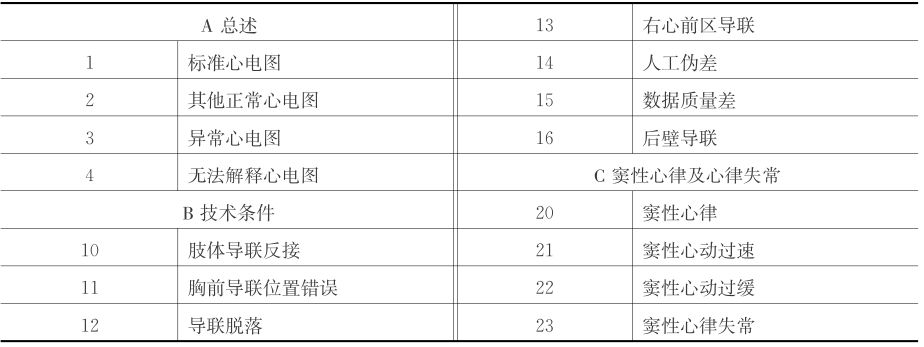
\includegraphics[width=\textwidth,height=\textheight,keepaspectratio]{./images/Image00747.jpg}\\
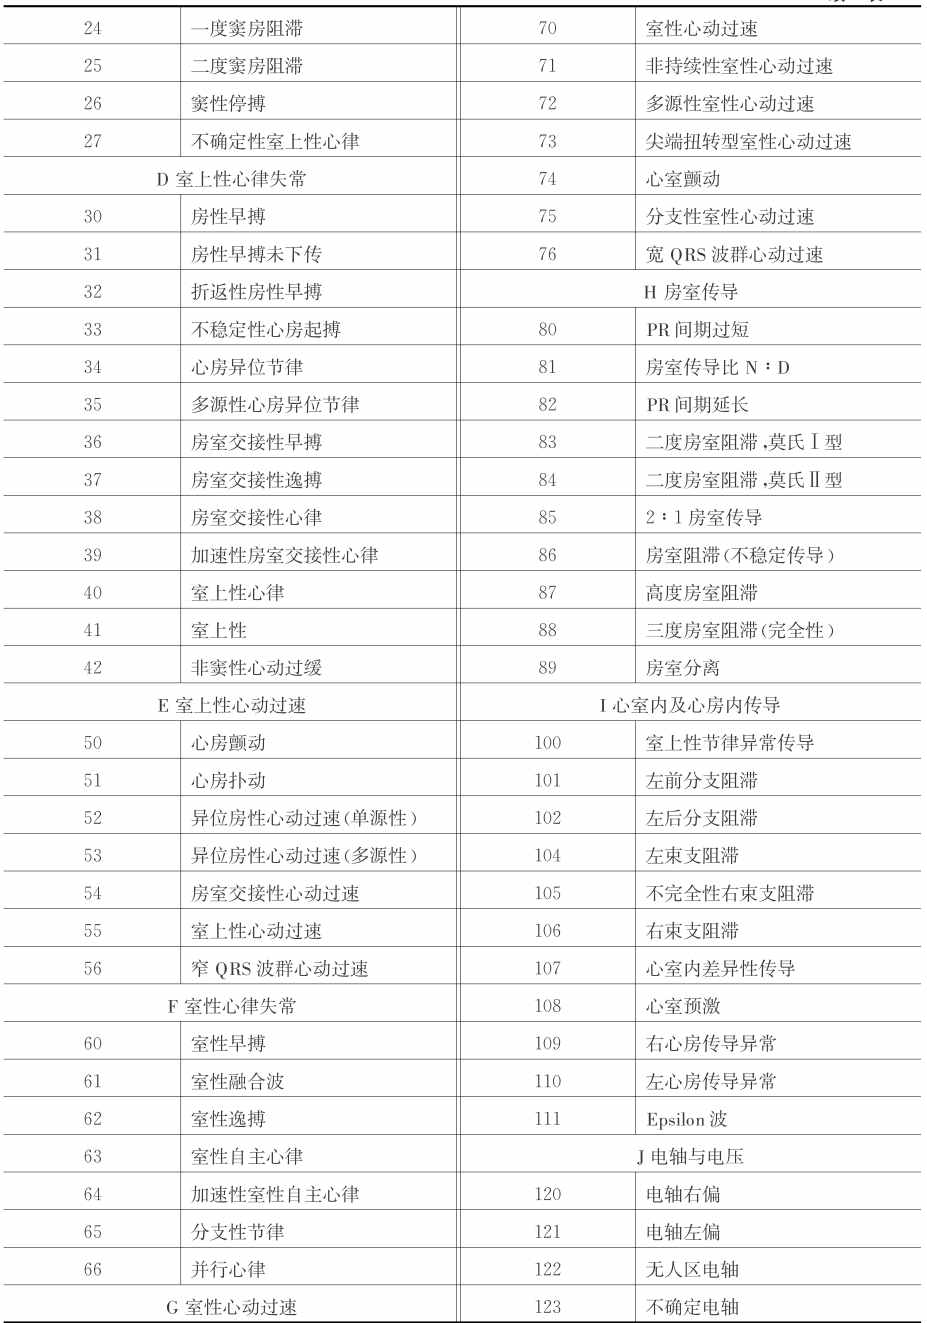
\includegraphics[width=\textwidth,height=\textheight,keepaspectratio]{./images/Image00748.jpg}\\
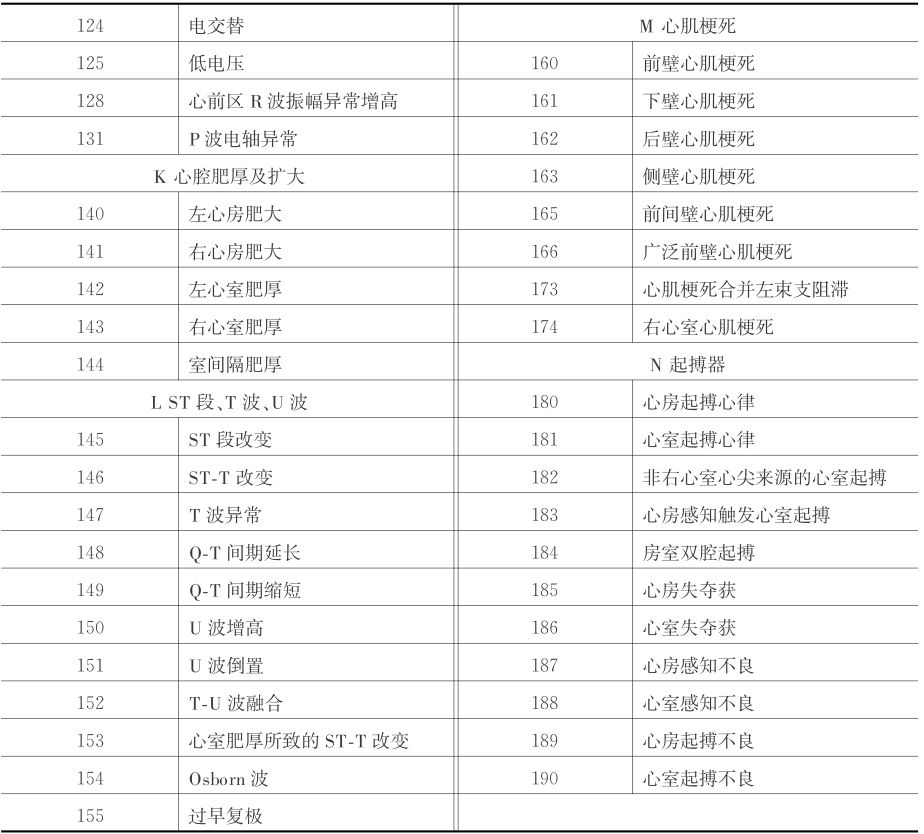
\includegraphics[width=\textwidth,height=\textheight,keepaspectratio]{./images/Image00749.jpg}
\end{longtable}

\protect\hypertarget{text00057.htmlux5cux23subid704}{}{}

\subsection{次要诊断术语}

次要诊断术语:结合临床,简单实用。分为建议性术语和考虑性术语两部分(表48-2),与首要诊断术语组成了“核心诊断术语”。共列出了27条与临床疾病、药物及电解质紊乱有关的诊断性名词。

\begin{longtable}{c}
  \caption{次要诊断术语}
  \label{tab48-2}\\
  \endfirsthead
  \caption[]{次要诊断术语}
  \endhead
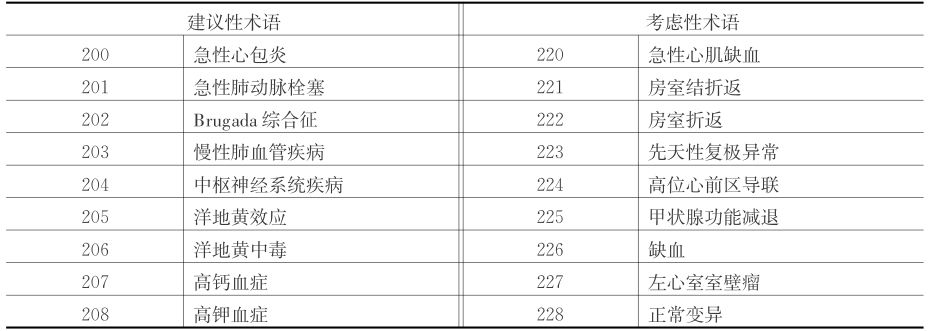
\includegraphics[width=\textwidth,height=\textheight,keepaspectratio]{./images/Image00750.jpg}\\
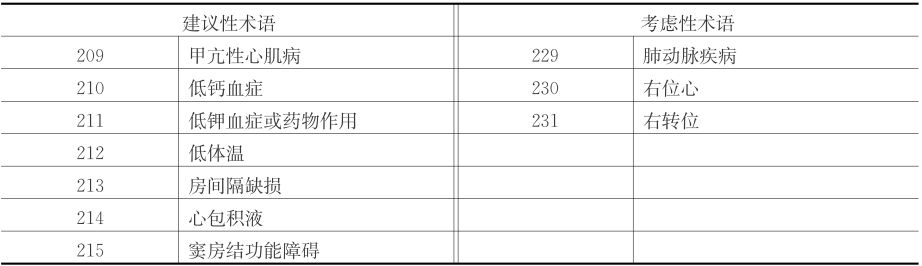
\includegraphics[width=\textwidth,height=\textheight,keepaspectratio]{./images/Image00751.jpg}
\end{longtable}

\subsection{修饰性词语}

修饰性词语用来修饰诊断术语,但不能改变核心术语的意义。共列出了47条修饰性词语。

\begin{table}[htbp]
\centering
\caption{修饰性词语}
\label{tab48-3}
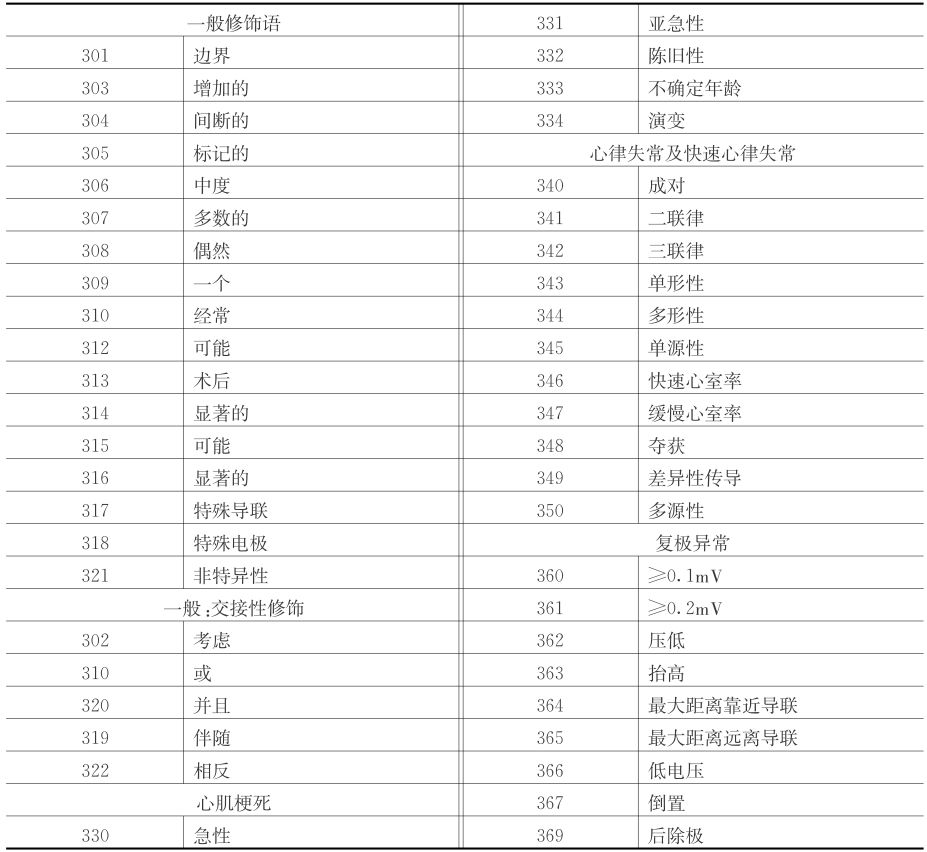
\includegraphics[width=5.44792in,height=5.01042in]{./images/Image00752.jpg}
\end{table}

\protect\hypertarget{text00057.htmlux5cux23subid706}{}{}

\subsection{比较性术语}

比较性术语:前后对照,发现新线索。共列出了6种值得注意的心电图改变,并制订了特定的心电图标准(表48-4)。

\begin{table}[htbp]
\centering
\caption{比较性术语}
\label{tab48-4}
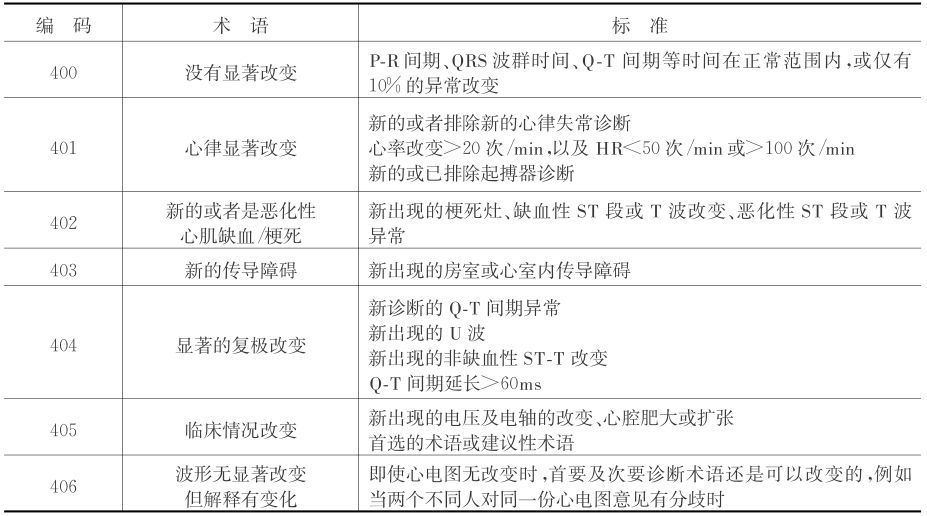
\includegraphics[width=5.44792in,height=3.03125in]{./images/Image00753.jpg}
\end{table}

\protect\hypertarget{text00057.htmlux5cux23subid707}{}{}

\subsection{一般使用规则}

心电图诊断时,只有首要诊断术语可以单独出现,而次要诊断术语和修饰性词语必须伴随首要诊断(表48-5)。

\begin{table}[htbp]
\centering
\caption{一般使用规则}
\label{tab48-5}
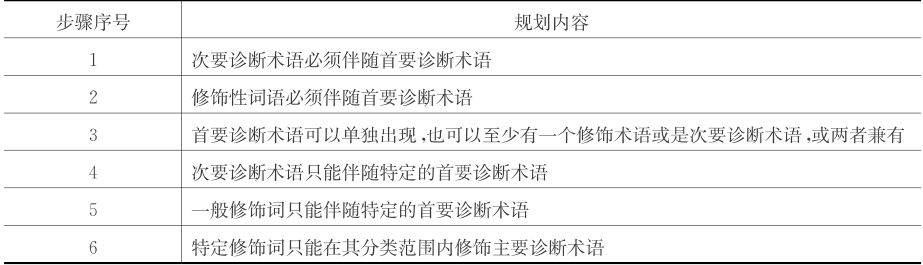
\includegraphics[width=6.23958in,height=1.79167in]{./images/Image00754.jpg}
\end{table}

\protect\hypertarget{text00057.htmlux5cux23subid708}{}{}

\subsection{术语配对规则}

指南中规定了首要与次要诊断术语配对规则、一般修饰性词语与首要诊断术语配对规则,使诊断主次分明、简单明了(表48-6、表48-7)。

\begin{longtable}{c}
  \caption{首要及次要诊断术语配对规则}
  \label{tab48-6}\\
  \endfirsthead
  \caption[]{首要及次要诊断术语配对规则}
  \endhead
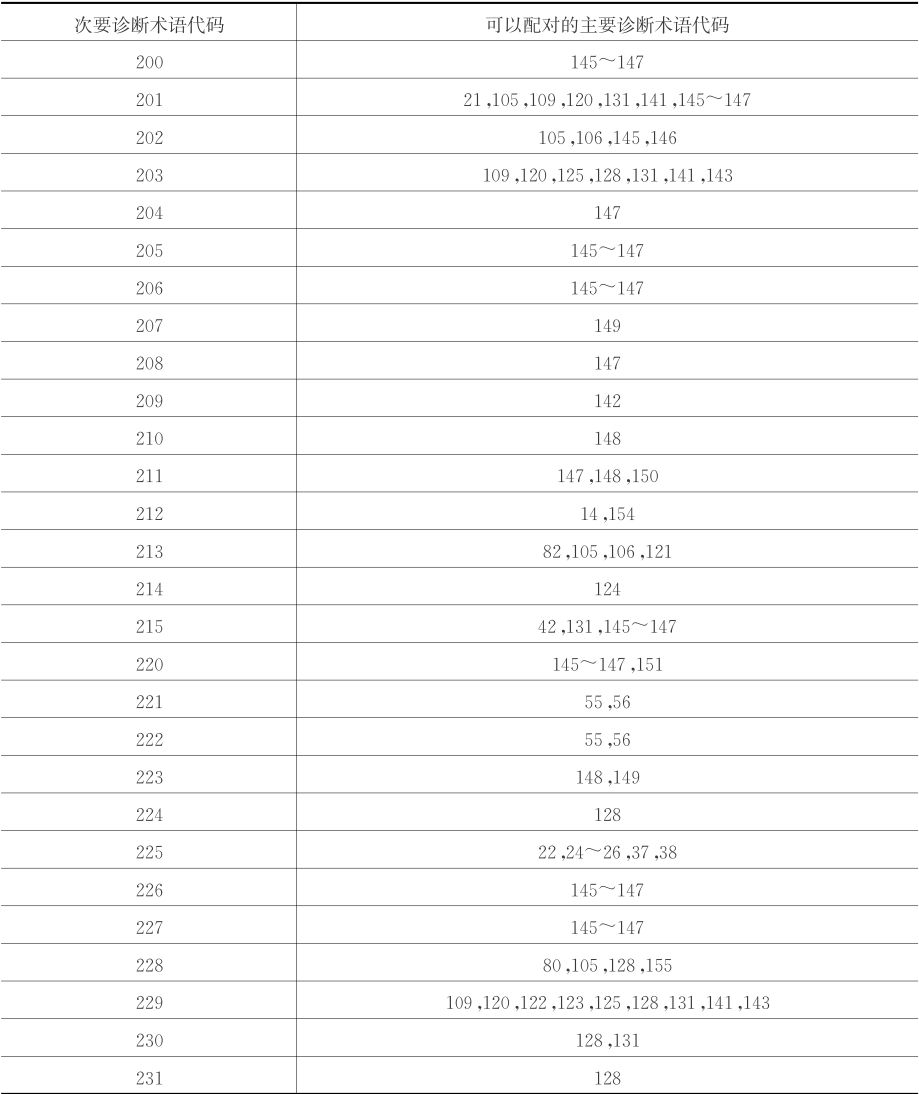
\includegraphics[width=\textwidth,height=\textheight,keepaspectratio]{./images/Image00755.jpg}
\end{longtable}

\begin{longtable}{c}
  \caption{一般修饰语与首要诊断术语配对规则}
  \label{tab48-7}\\
  \endfirsthead
  \caption[]{一般修饰语与首要诊断术语配对规则}
  \endhead
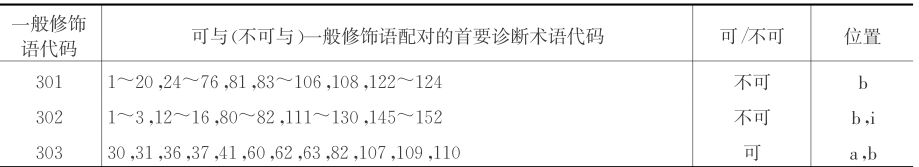
\includegraphics[width=\textwidth,height=\textheight,keepaspectratio]{./images/Image00756.jpg}\\
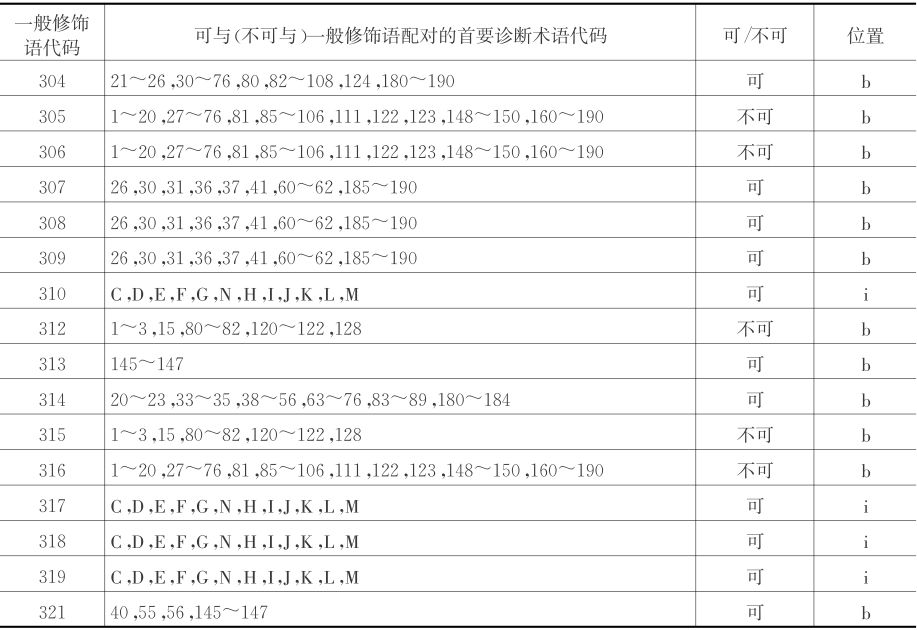
\includegraphics[width=\textwidth,height=\textheight,keepaspectratio]{./images/Image00757.jpg}
\end{longtable}

\protect\hypertarget{text00057.htmlux5cux23subid709}{}{}

\subsection{便捷性术语}

考虑到心电图的特殊性及与临床的相关性,指南中提出了4条便捷性术语(表48-8)。

\begin{table}[htbp]
\centering
\caption{便捷性术语}
\label{tab48-8}
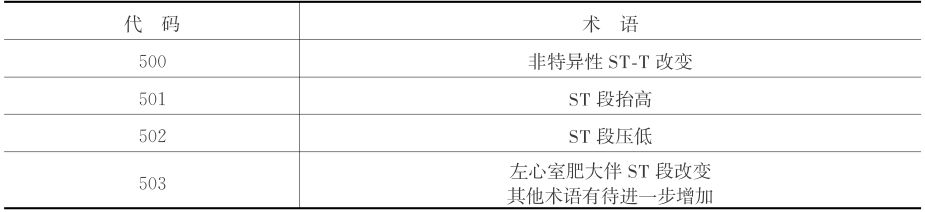
\includegraphics[width=5.4375in,height=1.23958in]{./images/Image00758.jpg}
\end{table}

申明:本节“2009年国际指南”内容是参阅了由中国心律学会编写的、由中国环境出版社出版的《心电图标准化和解析的建议与临床应用国际指南2009》一书,不知是翻译原因,还是编排原因,发现部分内容值得商榷,如代码24(一度窦房阻滞),体表心电图是无法直接诊断一度窦房阻滞的;代码41(室上性)、42(非窦性心动过缓),临床上是没有这种诊断术语的;代码312(可能)与315(可能)重复、代码314(显著的)与316(显著的)重复、代码310(经常)与310(或)重复出现且含义不同等。此外,本人对“2009年国际指南”的部分内容持有异议,如“心室肥厚”的名称及表48-6、表48-7的术语配对规则,过于繁杂。本人拟建的临床心电图诊断库则简明、实用,读者可明鉴。

\protect\hypertarget{text00058.html}{}{}

\protect\hypertarget{text00058.htmlux5cux23chapter58}{}{}

\chapter{如何撰写心电图案例分析}

\protect\hypertarget{text00058.htmlux5cux23subid710}{}{}

\subsection{选择合适的题材及图片}

1.博览群书及期刊

选择合适的题材及图片是撰写心电图案例分析的关键。与心血管病相关的杂志,尤其是《心电学杂志》、《临床心电学杂志》、《中国心脏起搏与电生理杂志》等期刊,每期均有不同篇幅的心电图案例分析。我们应该经常翻阅或上网查阅这些与本专业相关的杂志,以了解最新信息,帮助我们从日常工作中所遇到的各种各样图片中筛选出合适的题材。

2.适合撰写心电图案例分析的内容

撰写心电图案例分析最好是杂志上尚未报道或很少报道的内容和图片。有学者进行了回顾性归纳分类,大致有以下20余种情况可作为撰写心电图案例分析的内容:疑难心电图、复杂心电图、复合心电图、罕见现象、特殊类型、典型案例、正常变异、容易造成混淆不清的案例、需要鉴别诊断、内容新颖、有新见解、变化多端、一过性表现、隐而未见需要通过间接推断、有临床指导意义、有辅助诊断价值、有诱发因素、易误诊案例、药物或电解质影响及先天性畸形所致等,但其中以心律失常案例报道最为多见。

\protect\hypertarget{text00058.htmlux5cux23subid711}{}{}

\subsection{如何处置心电图图片}

心电图论文最大的特点是图文并茂。清晰的图片、简洁美观的梯形图解是文稿的重要组成部分,也反映了作者的思路,同时有助于读者的阅读和理解。

1.描记一幅美观清晰的心电图片子

(1)所描记的心电图必须基线平稳、无伪差波,各波段的波形清晰、粗细均匀。

(2)选择心房波(P波、F波或f波)清晰的导联,必要时加做S\textsubscript{5}
、食道导联,一般选择Ⅱ、V\textsubscript{1} 、V\textsubscript{5}
导联,最好是同步记录。

(3)选择与文稿内容密切相关的导联或片段加以整理:①12导联剪贴时包括1个完整的心动周期,即包含P-QRS-T-U波群,心率较快时可包括2~3个心动周期。②最好保持每一片段大小一致,尤其是每行的高度应该一致,以各个片段中QRS波群电压最高者为准,每一个片段都要严格按照背景方格剪取,一丝不苟。③酌情横贴,如肢体导联(Ⅰ、Ⅱ、Ⅲ、aVR、aVL、aVF)贴上行,胸前导联(V\textsubscript{1}
~V\textsubscript{6}
)贴下行;或者竖贴,如Ⅰ、Ⅱ、Ⅲ导联竖贴一行,aVR、aVL、aVF导联竖贴一行,V\textsubscript{1}
、V\textsubscript{2} 、V\textsubscript{3}
导联竖贴一行,V\textsubscript{4} 、V\textsubscript{5}
、V\textsubscript{6}
导联竖贴一行;粘贴时,行间、列间均应保留1mm左右的间隙,为保证粘贴整齐不歪斜,先在白纸上画好暗线,逐一紧贴其左缘、下缘粘贴上。④有关心律失常图片,必须连续记录适当的长度,如文氏现象至少应显示2~3个完整的文氏周期,并行心律应显示5个以上异位搏动\ldots{}\ldots{}每行的长度以16~20cm为宜。⑤需绘制梯形图解者,应在长行心电图下方1~2mm处,按照绘制梯形图解技巧要求绘制。⑥切勿直接在图片上写上各种符号,如导联、数字等,可在图片要标记地方的上方、下方或左方等处用铅笔标上。

(4)图片复印时,必须选择高质量的复印机,选择合适的复印浓度,使图片清晰,浓淡适中。

\protect\hypertarget{text00058.htmlux5cux23subid712}{}{}

\subsection{文题命名及撰写格式}

(1)文题命名:必须要求题意新颖、紧扣或能概括心电图的主要诊断,并且文字不宜过长(一般少于20个字)。

(2)撰写格式:一般按照前言或引言、病历摘要(主诉、体检、相关的辅助检查及临床诊断)、心电图特点描述及分析、心电图诊断、讨论及分析相关内容、得出某种有价值的结论性意见、参考文献等顺序进行撰写。

\protect\hypertarget{text00058.htmlux5cux23subid713}{}{}

\subsection{如何描述心电图特点}

(1)先对常规12导联心电图的基本节律、频率、各个波段有无异常改变进行描述,借以确定基本节律是什么,有无房室肥大、传导阻滞及ST段、T波、U波改变等。

(2)描述连续记录的心律失常图片,着重描述与心律失常相关的心电图特点,同时根据该特点推理是哪种性质的心律失常。

(3)结合临床资料,必要时与过去的心电图片子相比较,给该幅图片下一个完整而确切的心电图诊断。

\protect\hypertarget{text00058.htmlux5cux23subid714}{}{}

\subsection{讨论内容的撰写}

讨论内容是论文的重点内容,可以是紧扣心电图主要诊断加以引申,如该诊断的诊断条件或标准,需作哪些鉴别诊断及其鉴别要点;也可以是引用他人的观点,对某一心律失常的心电图表现及其类型、发生机制、诊断条件或标准、临床意义及转归等内容进行讨论。要求文字简明扼要,精练通顺,重点突出,全文控制在1500个字以内。

\protect\hypertarget{text00058.htmlux5cux23subid715}{}{}

\subsection{参考文献的引用}

选择最近5年内与本文内容相关的各种期刊、书籍作为参考文献,按照文中出现的先后按次序予以引出,一般引用5篇左右即可。

\protect\hypertarget{text00059.html}{}{}

\protect\hypertarget{text00059.htmlux5cux23chapter59}{}{}

\chapter{疑难心电图精解20例}

例1 室性早搏伴折返径路内A型交替性反向文氏周期

【临床资料】

患者男性,32岁,临床诊断:病毒性心肌炎。

\begin{figure}[!htbp]
 \centering
 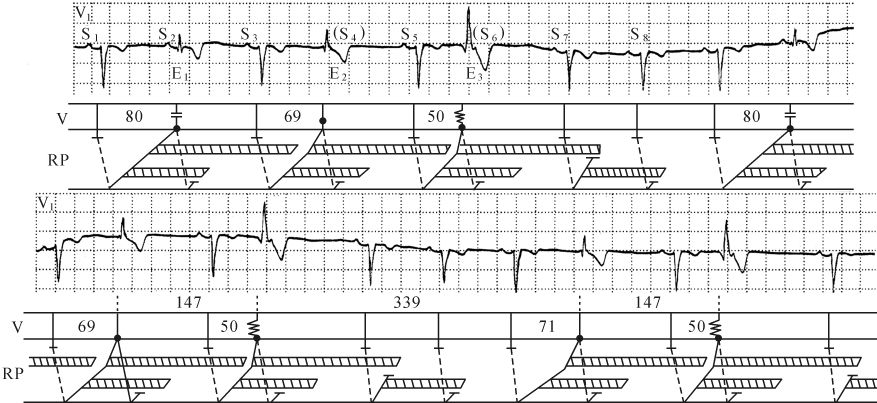
\includegraphics[width=5.92708in,height=2.71875in]{./images/Image00759.jpg}
 \captionsetup{justification=centering}
 \caption{例1 室性早搏伴折返径路内A型交替性反向文氏周期}
 \label{fig50-1}
  \end{figure} 

【心电图特征】

V\textsubscript{1}
导联连续记录,示QRS波形有4种:①呈rS型,P-R间期0.14s,为窦性激动下传心室;②呈qrs型,P-R间期0.11s,为室性融合波,如E\textsubscript{1}
;③呈qR型,提早出现,其前无P波,系室性早搏,如E\textsubscript{2}
;④也呈qR型,发生在长-短周期之后,符合室性早搏伴心室内差异性传导,如E\textsubscript{3}
。室性早搏的偶联间期由0.80s→0.69s→0.50s→早搏消失,连续出现3次窦性搏动,周而复始,显示室性早搏伴折返径路内A型交替性反向文氏周期。

【精解与讨论】

梯形图RP行斜线区代表有效不应期的长短,虚线表示窦性激动进入折返径路前的心室内传导,实线表示折返径路。本例折返径路近端的有效不应期稍长于1个窦性周期,远端的有效不应期短于窦性周期的2倍,窦性激动S\textsubscript{1}
、S\textsubscript{3} 和S\textsubscript{5}
通过折返径路折回心室,分别引起偶联间期0.80s、0.69s和0.50s的室性融合波E\textsubscript{1}
、室性早搏E\textsubscript{2} 和E\textsubscript{3}
,表明激动在穿越折返径路远端阻滞区的速度逐渐加快,以致S\textsubscript{5}
激动折回心室时,心室内传导组织、心室肌尚未完全脱离不应期,导致室性早搏E\textsubscript{3}
发生心室内差异性传导。E\textsubscript{1} 、E\textsubscript{2}
、E\textsubscript{3}
的激动又进入折返径路,但在近端被阻滞,当S\textsubscript{7}
激动折回心室时,因传导速度加快在远端遇及前一激动的有效不应期而阻滞,下一个激动S\textsubscript{8}
则被阻滞在近端。故窦性激动如S\textsubscript{1} 、S\textsubscript{3}
、S\textsubscript{5} 和S\textsubscript{7}
在折返径路远端发生4:3传出反向文氏现象,下行最后一个文氏周期远端为3:2传出阻滞,说明折返径路内有两个水平阻滞区,即近端2:1阻滞,远端3:2~4:3传出反向文氏现象,符合A型交替性反向文氏周期。

因心室肌不应期甚短,室性早搏不易产生心室内差异性传导,但一旦出现,则提示心肌有病变。本例系病毒性心肌炎患者,室性早搏发生心室内差异性传导,表明心室内传导组织、心室肌受炎症影响,其不应期出现病理性延长,这更有利于折返性早搏的形成。

本例应与下列心律失常相鉴别:①偶联间期反向文氏型室性并行心律:当两个室性早搏的间距为并行灶的基本周期,且稍短于2个窦性周期时,则每个室性早搏愈来愈接近前面的窦性搏动,直至落到前一个窦性搏动后的绝对不应期内而消失,貌似折返径路内反向文氏现象;但并行心律属起源异常,与其前配对的心搏无关,两个室性早搏之间的距离相等或呈倍数关系,仍保持并行心律的特点;本例两个室性早搏的间距不等,亦不呈倍数关系,可排除偶联间期反向文氏型并行心律。②室性并行心律伴文氏型传出阻滞:表现为偶联间期长短无规律地改变,两个相邻室性早搏的E-E间期呈渐短突长,长E-E间期短于最短E-E间期的2倍;本例室性早搏的偶联间期由长到短有规律地改变,尔后出现固定偶联间期,表明室性早搏与其前配对的心搏有关,属传导异常;此外,最长E-E间期3.39~3.45s,大于最短E-E间期1.47s的2倍,故本例可除外室性并行心律伴文氏型传出阻滞。③多源性室性早搏:属起源异常,其偶联间期、QRS波形均不一致,本例虽然早搏偶联间期、QRS波形不一致,但偶联间期由长到短有规律地变化,故仍考虑为传导异常,可除外多源性室性早搏。④异位起搏点自律性强度不等引起偶联间期长短不一:属起源异常,当异位灶的自律性增强时,其发放频率加快,表现为短的偶联间期;当自律性强度减低时,其发放频率减慢,则出现长的偶联间期,但像本例偶联间期由长到短有规律地改变,是非常罕见的。

【心电图诊断】

①窦性心律;②频发室性早搏,呈显性、隐性二联律,有时伴心室内差异性传导;③室性融合波;④心室折返径路内A型交替性反向文氏周期(近端2:1阻滞,远端3:2~4:3反向文氏现象)。

例2 窦性早搏二联律伴3相性右束支阻滞及室性早搏四联律

【临床资料】

患者男性,34岁,临床诊断:病毒性心肌炎。

【心电图特征】

V\textsubscript{3} 导联连续记录,P\textsubscript{15}
-P\textsubscript{16}
间期1.09s为窦性基本周期,提早出现的P′\textsubscript{4}
、P′\textsubscript{8} 、P′\textsubscript{12}
的形态与窦性P波一致,偶联间期0.74~0.76s,代偿间歇1.01~1.09s呈次等周期、等周期代偿,下传的QRS波群呈右束支阻滞型(时间0.15s);提早出现的R\textsubscript{2}
、R\textsubscript{6} 、R\textsubscript{10} 、R\textsubscript{14}
呈左束支阻滞型(时间0.16s),偶联间期0.44s,代偿间歇不完全。

【精解与讨论】

窦性早搏的诊断条件:①提早出现的P′波形态与窦性P波一致或略异;②P′-P间期等于窦性P-P间期,呈等周期代偿。

窦房交接性早搏的诊断条件:①提早出现的P′波形态与窦性P波一致或略异;②可呈次等周期、等周期代偿或不完全性代偿间歇。

本例短P-P′间期0.74~0.76s与长P′-P间期1.01~1.09s交替出现呈二联律,但最后1个窦性周期1.09s与长P′-P间期相等。按照Schamroth的意见,如果所显现的窦性心律其P-P间期与二联律时的长P-P间期相等,则此二联律为窦性早搏二联律。本例代偿间歇1.01~1.09s表现为次等周期或等周期代偿,是窦性心律不齐所致,还是窦性早搏触发窦性节律提早发放或窦房交接性早搏在窦房交接区前向、逆向传导速度发生改变所致?尚难肯定。室性早搏的代偿间歇往往是完全的,本例室性早搏的QRS波群后面无逆行P\textsuperscript{-}
波跟随而呈不完全代偿间歇,显然要考虑窦性早搏的P′波重叠于室性早搏的QRS波群中,两者在房室交接区产生相互干扰。

\begin{figure}[!htbp]
 \centering
 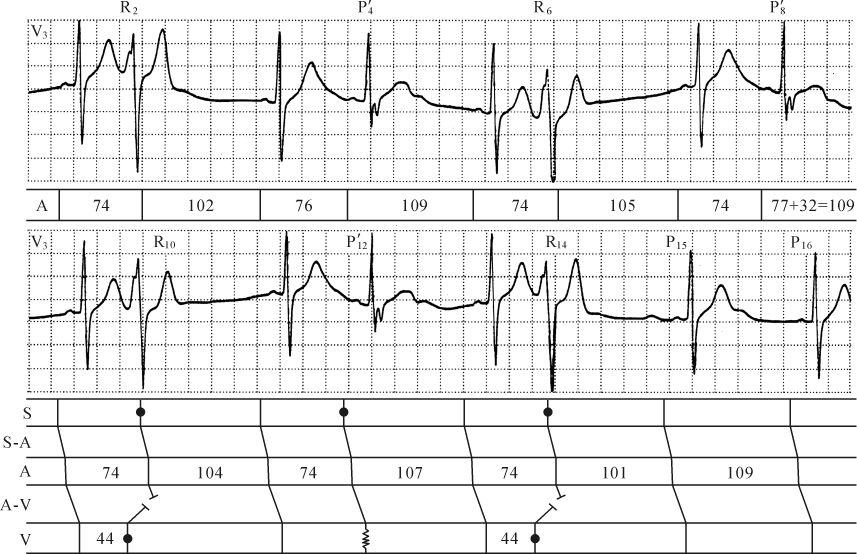
\includegraphics[width=5.79167in,height=3.73958in]{./images/Image00760.jpg}
 \captionsetup{justification=centering}
 \caption{例2 窦性早搏二联律伴3相性右束支阻滞及室性早搏四联律}
 \label{fig50-2}
  \end{figure} 

本例应与下列心律失常相鉴别:①房性早搏二联律:房性早搏的P′波形态异于窦性P波,早搏后代偿间歇P′-P间期等于窦性P-P间期加上心房冲动到窦房结的传导时间(P′-S)和窦性冲动传到心房的时间(S-P)而呈不完全代偿间歇。②3:2窦房文氏现象:短P-P间期与长P-P间期交替出现呈二联律时,若无窦性心律显现,3:2窦房文氏现象与窦性早搏二联律无法区别;若所显现的窦性心律,其P-P间期小于二联律时的较短P-P间期,则为前者;若P-P间期等于较长P-P间期,则为后者。③窦房交接区快、慢径路交替传导:二联律时长、短P-P间期之和为二联律消失时所显现的窦性心律基本P-P间期的2倍,经快径路传导时出现短P-P间期,由慢径路传导时出现长P-P间期。

【心电图诊断】

①窦性心律;②频发窦性早搏或窦房交接性早搏二联律伴3相性右束支阻滞;③频发室性早搏四联律;④窦性早搏或窦房交接性早搏与室性早搏在房室交接区出现相互干扰现象。

例3 双束支阻滞、房室交接性逸搏心律合并左束支内文氏现象

【临床资料】

患者男性,81岁,临床诊断:冠心病。

【心电图特征】

V\textsubscript{1}
-a导联P-P间期0.78~0.82s,P-R间期0.18s,P波与QRS波群呈2:1传导,QRS波群呈RsR′型,时间0.12~0.13s,为完全性右束支阻滞。V\textsubscript{1}
-b、V\textsubscript{1}
-c导联连续记录(定准电压0.5mV),P-P间期0.81s,除R\textsubscript{1}
、R\textsubscript{5}
搏动呈右束支阻滞型及其P-R间期固定为0.18s外,其余搏动的QRS波群呈rS型,其P-R间期均不固定,表明P波与QRS波群无关,R-R间期1.42~1.46s,时间由0.11s→0.12s→0.16s逐渐增宽,表现为左束支内文氏现象。

\begin{figure}[!htbp]
 \centering
 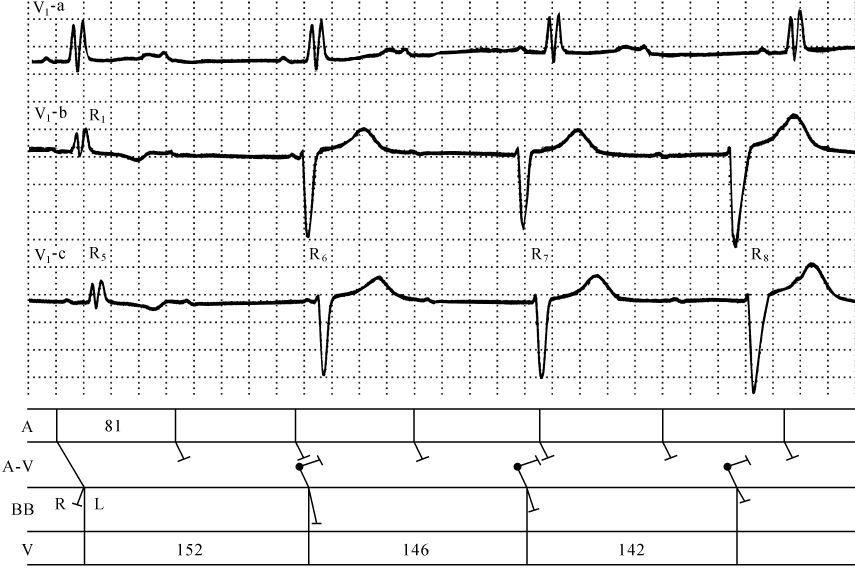
\includegraphics[width=5.78125in,height=3.85417in]{./images/Image00761.jpg}
 \captionsetup{justification=centering}
 \caption{例3 双束支阻滞、房室交接性逸搏心律合并左束支内文氏现象}
 \label{fig50-3}
  \end{figure} 

【精解与讨论】

常见的双束支及双分支阻滞心电图表现有以下6种类型:①完全性右束支阻滞伴左前分支阻滞;②完全性右束支阻滞伴左后分支阻滞;③间歇性出现右、左束支阻滞;④间歇性出现左前、左后分支阻滞;⑤完全性左束支阻滞合并房室传导阻滞型(P-R间期延长、二度Ⅰ型、二度Ⅱ型房室传导阻滞,考虑其阻滞部位发生在右束支内);⑥一部分完全性右束支阻滞合并房室传导阻滞型(P-R间期延长、二度Ⅰ型、二度Ⅱ型房室传导阻滞,考虑其阻滞部位发生在左束支内)。本例V\textsubscript{1}
-a导联在完全性右束支阻滞基础上出现2:1房室传导阻滞,该阻滞部位可能发生在房室结或左束支内,结合V\textsubscript{1}
-b、V\textsubscript{1}
-c导联出现二度或高度房室传导阻滞,提示V\textsubscript{1}
-a导联2:1房室传导阻滞的部位发生在房室结内。

窦性激动下传心室时,诊断束支内文氏现象的前提为:①要求P-P间期规则以排除频率依赖性束支阻滞;②要求P-R间期固定及≥0.12s以排除室性逸搏、室性融合波及预激综合征。束支内文氏现象有3种类型:①直接显示型:QRS波形由正常→不完全性束支阻滞→完全性束支阻滞逐渐演变,周而复始;②不完全性隐匿型:QRS波形表现为不完全性束支阻滞→完全性束支阻滞,周而复始;③完全隐匿型:QRS波群呈完全性束支阻滞型,时间固定不变或逐渐增宽,要诊断该型,需同时存在直接显示型或不完全性隐匿型方可诊断,否则,与一般的完全性束支阻滞无法区别。

本例V\textsubscript{1} -b、V\textsubscript{1}
-c导联初看酷似高度房室传导阻滞,结合V\textsubscript{1}
-a导联,实际上亦为2:1房室传导阻滞,P波落在左束支阻滞型QRS波群稍前、之中及T波上升肢上均系生理性干扰所致。从梯形图解中可知,R\textsubscript{5}
为窦性激动经左束支下传,R\textsubscript{6} 、R\textsubscript{7}
为不完全性左束支阻滞型,系房室交接性逸搏由右束支下传心室,其左、右束支传导时间互差0.025~0.04s,R\textsubscript{8}
呈完全性左束支阻滞型,为房室交接性逸搏经右束支下传,其左、右束支传导时间互差>0.04s,表明左束支阻滞程度逐渐加重,提示房室交接性逸搏心律合并直接显示型左束支内4:3文氏现象。

本例双束支阻滞系功能性阻滞所致,即由左、右束支传导时间互差>0.04s所致。需与双源性室性逸搏伴室性融合波相鉴别,即V\textsubscript{1}
-c导联的R\textsubscript{6} 为高位室性逸搏,R\textsubscript{8}
为低位室性逸搏,R\textsubscript{7}
为两者的室性融合波,根据QRS波形有规律地重复出现,以房室交接性逸搏心律合并左束支内文氏现象可能性为大。

【心电图诊断】

①窦性心律;②二度房室传导阻滞,房室呈2:1传导;③完全性右束支阻滞;④房室交接性逸搏心律合并直接显示型左束支内4:3文氏现象;⑤窦性激动与房室交接性逸搏在交接区发生干扰现象酷似高度房室传导阻滞。

例4 加速的房室旁道性逸搏心律

【临床资料】

患者女性,14岁,临床诊断:病毒性心肌炎?

\begin{figure}[!htbp]
 \centering
 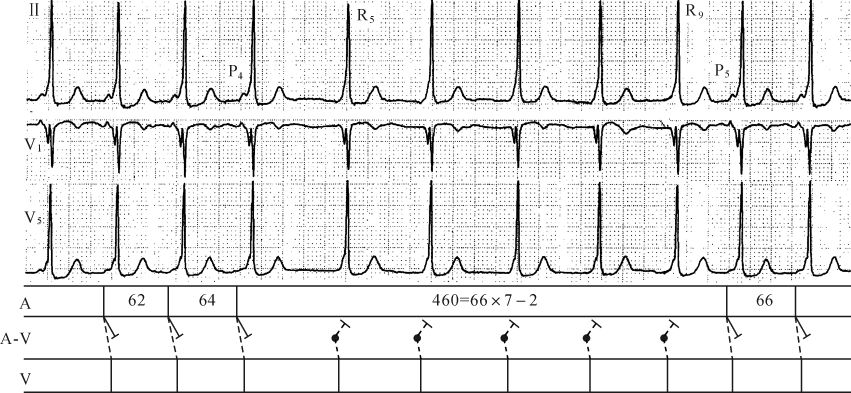
\includegraphics[width=5.75in,height=2.65625in]{./images/Image00762.jpg}
 \captionsetup{justification=centering}
 \caption{例4 加速的房室旁道性逸搏心律}
 \label{fig50-4}
  \end{figure} 

【心电图特征】

Ⅱ、V\textsubscript{1} 、V\textsubscript{5}
导联同步记录,P-P间期0.62~0.66s,P\textsubscript{4} -P\textsubscript{5}
间期4.60s,为部分短P-P间期的7倍,P-R间期0.08s,QRS波群落在P波的下降肢上,无PR段,QRS波群时间0.12s,有“δ”波,V\textsubscript{1}
导联呈QS型,起始错折或呈qrS型,V\textsubscript{5}
导联呈R型,提示为完全性B型预激综合征;值得注意的是R\textsubscript{5}
~R\textsubscript{9}
的形态与其他QRS波形完全一致,但其前均未见任何P波,R-R间期0.71~0.80s,频率75~84次/min,应考虑为起源于Kent束的加速的逸搏心律(梯形图A-V行中实线表示房室正道,虚线表示房室旁道)。

【精解与讨论】

大部分Kent束顺向传导不应期极短≤0.35s,称为快旁道,由心房肌构成,无自律性,传导具有全或无特性,无递减性传导或传导延缓,不存在一度或文氏型阻滞;小部分Kent束不应期相当长,可在0.60~3.0s,称为慢旁道,是由希-浦传导组织构成,具有自律性。现已证明,在旁道束纤维内或旁道束插入心房和心室的部位均易产生异位激动,所形成的早搏大多以并行节奏点的性质单个出现,有时亦可形成异位心律;亦可有3相、4相阻滞及超常传导。

本例加速的旁道性逸搏心律应与下列心律失常相鉴别:①加速的房性逸搏心律伴B型预激:若心房异位灶接近旁道束的起始部且优先由旁道束下传心室,而激动传向心房肌受阻,未使心房肌除极产生P′波或所产生P′波振幅极低或与窦性P波相融合形成房性融合波重叠在等电位线上难以分辨,但在Ⅱ、V\textsubscript{1}
、V\textsubscript{5}
三个导联上均未见P′波或房性融合波则难以解释,故可排除。②加速的室性逸搏心律:若心室异位灶接近旁道束插入心室部位时,则两者因QRS波形相似在体表心电图上无法鉴别,若异位灶起源于心室其他部位,则因QRS波形不一而可排除。③加速的房室交接性逸搏或室性逸搏心律伴完全性房室分离:心房由窦性控制,心室由房室交接区或室性异位搏动控制,P波与QRS波群无关呈完全性房室分离,但常规十二导联及Ⅱ、V\textsubscript{1}
、V\textsubscript{5}
导联同步记录时,即使P-P间期不等,其P-R间期始终是固定的,表明P波与QRS波群是相关的,故可排除。

【心电图诊断】

①窦性心律;②高度窦房传导阻滞;③完全性B型预激综合征;④加速的房室旁道性逸搏心律。

例5 室性并行灶周围显性折返伴折返径路内反向文氏现象

【临床资料】

患者男性,72岁,临床诊断:冠心病?

\begin{figure}[!htbp]
 \centering
 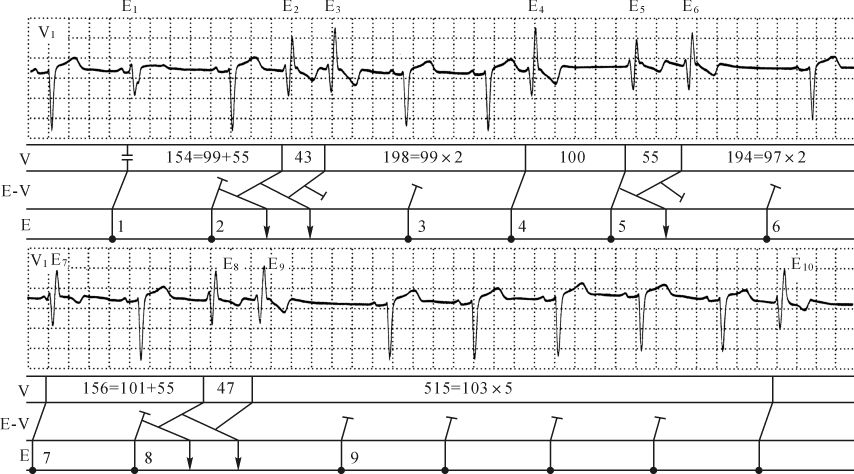
\includegraphics[width=5.77083in,height=3.19792in]{./images/Image00763.jpg}
 \captionsetup{justification=centering}
 \caption{例5 室性并行灶周围显性折返伴折返径路内反向文氏现象}
 \label{fig50-5}
  \end{figure} 

【心电图特征】

V\textsubscript{1}
导联连续记录,心电图有以下特点:①室性早搏的偶联间期不等,E\textsubscript{1}
为室性融合波,E\textsubscript{3} 、E\textsubscript{4}
R′振幅稍高,可能伴有轻度的心室内差异性传导;②成对室性早搏的E-E间期为0.43s、0.47s,连续出现3次异位搏动的E-E间期为1.00s、0.55s;③其余相邻的两个异位搏动的E-E间期分别为1.54s、1.98s、1.94s、1.56s、5.15s。

【精解与讨论】

室性并行灶周围显性折返伴折返径路内反向文氏现象的心电图诊断条件:①异位搏动的偶联间期不等;②有多个成对早搏,其E-E间期为显性折返周期,并且由长到短,直至异位搏动消失,且能重复出现;③长E-E间期不是成对早搏E-E间期的倍数,而是所测得并行灶基本周期的倍数和余数,其余数为成对早搏E-E间期的倍数。

从梯形图解中可知,长E-E间期1.94s、1.98s、5.15s为0.97~1.03s的2~5倍,故E\textsubscript{4}
-E\textsubscript{5}
间期1.00s即为并行灶的基本周期。长E-E间期1.54s、1.56s不是成对室性早搏E-E间期0.43s、0.47s的倍数,而是并行灶基本周期的长度加上余数0.55s,而余数恰好与E\textsubscript{5}
-E\textsubscript{6}
间期相等,故0.55s为显性折返周期,表明E\textsubscript{5}
外出时在并行灶周围产生折返并重整并行灶节律,同时亦传出心室形成折返心搏E\textsubscript{6}
;并行灶发放的第2、8个激动(梯形图E行中所标的2、8数字)外出时,恰逢心室肌处于窦性搏动后的绝对不应期而未传出,但在并行灶周围产生连续数次折返并激动心室形成显性折返心搏E\textsubscript{2}
、E\textsubscript{3} 及E\textsubscript{8} 、E\textsubscript{9}
,且重整并行灶节律,折返激动在并行灶周围的折返径路内传导速度逐渐加快,引起折返心搏E-E间期由0.55s→0.43~0.47s,逐渐缩短,直至第3次折返激动遇及心室肌、并行灶节律点的不应期而终止,显示并行灶周围折返径路内呈2:1~3:2反向文氏现象。

【心电图诊断】

①窦性心律;②频发单个、成对室性早搏;③短阵性室性心动过速;④室性并行灶周围显性折返伴折返径路内2:1~3:2反向文氏现象。

例6 室性并行心律伴并行灶周围传导3种可能

【临床资料】

患者男性,62岁,临床诊断:冠心病。

\begin{figure}[!htbp]
 \centering
 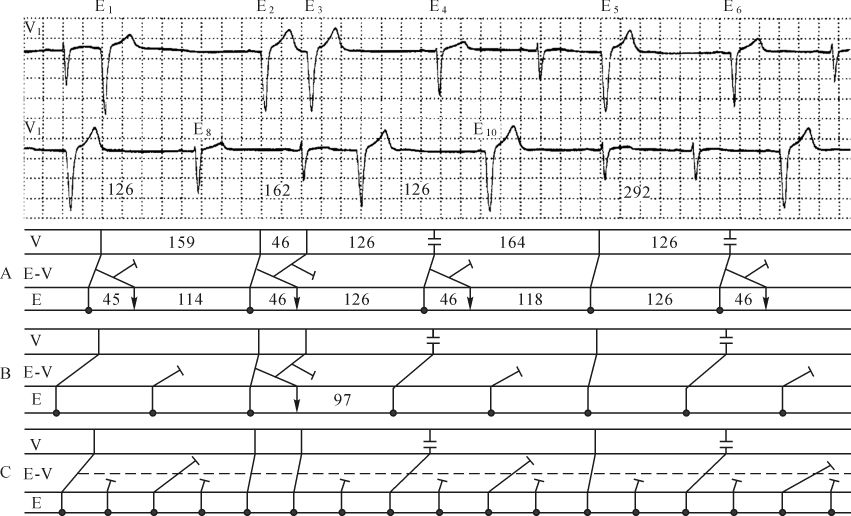
\includegraphics[width=5.75in,height=3.48958in]{./images/Image00764.jpg}
 \captionsetup{justification=centering}
 \caption{例6 室性并行心律伴并行灶周围传导3种可能(梯形图解按上行V\textsubscript{1}}
 \label{fig50-6}
  \end{figure} 
导联绘制)

【心电图特征】

V\textsubscript{1}
导联连续记录(定准电压0.5mV),示窦性P-P间期0.91~1.05s,QRS波形有3种:①呈rS型,P-R间期0.17s,系窦性搏动;②呈QS型,时间0.12s,其前无P波或相关P波,属室性异位搏动;③呈rS型,形态介于上述两者之间,其P-R间期0.15~0.16s,为室性融合波,如E\textsubscript{4}
、E\textsubscript{6} 、E\textsubscript{8}
。室性异位搏动有3个特点:①偶联间期不等(0.38~0.88s),部分以逸搏形式出现;②频发室性融合波;③相邻的两个异位搏动的E-E间期为0.46s、1.26s、1.59~1.64s、2.92s,大部分以1.26s、1.59~1.64s交替出现。

【精解与讨论】

根据这3个特点,此幅心电图有以下3种解释:①室性并行心律伴并行灶周围显性和隐性折返:长E-E间期1.26s、1.59~1.64s、2.92s不是成对早搏E\textsubscript{2}
-E\textsubscript{3}
间期0.46s的倍数,而是并行灶基本周期1.14~1.26s的倍数(1~2倍)和余数,其余数0.45~0.46s恰好等于成对早搏E\textsubscript{2}
-E\textsubscript{3}
间期,符合并行灶周围显性和隐性折返(见梯形图解A)。并行灶最大公约数的均值为(最大值+最小值)÷2=(1.26+1.14)÷2=1.20s,均值变异范围=(均值-最小值)÷均值×100\%=(1.20-1.14)÷1.20×100\%=5\%,符合并行心律的特点。异位搏动E\textsubscript{1}
、E\textsubscript{4} 、E\textsubscript{6}
外出时,在保护性阻滞区内发生折返,该折返激动因遇及阻滞区外围组织尚处于前一次激动的不应期而未能传出保护性阻滞区,形成隐匿性折返,但该折返激动却穿过并行灶使其节律重整;E\textsubscript{2}
外出时,在保护性阻滞区内所产生的折返激动,则传出了心室而形成显性折返心搏E\textsubscript{3}
,同时亦重整了并行灶节律。其折返环路为并行灶→并行灶邻近组织(保护性阻滞区内)→并行灶→心室(显性折返)或并行灶邻近组织(隐匿性折返)。②室性并行心律伴并行灶周围显性折返和外出3:2文氏现象:并行灶的基本周期为(1.26+1.64)÷3=0.97s,异位激动E\textsubscript{2}
外出时,在保护性阻滞区内产生折返,该折返激动适逢心室肌处于应激期而传出保护性阻滞区激动心室,形成显性折返心搏E\textsubscript{3}
,同时穿过并行灶使其节律重整,最后一组文氏周期呈3:2顿挫型文氏现象(见梯形图解B)。③室性并行心律伴外出交替性A型文氏周期:根据各组文氏周期的长度可推算出异位搏动的基本周期为(1.26+1.64)÷3=0.957s、(1.26+1.62)÷3=0.96s、2.92÷3=0.97s,基本上为最短E-E间期0.46s的2倍,故异位灶发放激动的基本周期为0.46~0.49s,其均值为(0.46+0.49)÷2=0.475s,均值变异范围为(最大值-均值)÷均值=(0.49-0.475)÷0.475×100\%=3.2\%,符合并行心律的特点。因此,本例亦符合室性并行灶周围外出交替性A型文氏周期,即并行灶发放激动在外出过程中,近端呈2:1阻滞,远端发生3:2文氏现象(见梯形图解C)。确定并行灶的基本周期是本例明确诊断的关键。

【心电图诊断】

①窦性心律;②频发室性早搏、加速的室性逸搏及室性融合波,有时呈短阵性室性异位心律;③室性并行灶周围显性和隐性折返或并行灶周围显性折返及外出3:2文氏现象或并行灶周围外出交替性A型文氏周期。

例7 室性并行灶周围外出交替性A型文氏周期

【临床资料】

患者男性,62岁,临床诊断:直肠癌、冠心病?

【心电图特征】

心电图Ⅱ、Ⅲ导联系手术前同时记录,示有3个节律点控制心室:①Ⅱ导联R\textsubscript{4}
、R\textsubscript{8} 及Ⅲ导联R\textsubscript{6}
,其前有窦性P波,P-R间期0.12s,为窦性搏动,其P-P间期规则1.04s,频率58次/min;②Ⅱ导联R\textsubscript{2}
、R\textsubscript{6} 及Ⅲ导联R\textsubscript{1} 、R\textsubscript{3}
、R\textsubscript{7}
QRS波群延迟出现,其形态与窦性一致,逸搏周期0.80s、0.89s、1.19s,频率50~75次/min,两异位搏动之间无最大公约数,属房室交接性逸搏或加速的房室交接性逸搏;③Ⅱ导联提早或延迟出现的呈R型及Ⅲ导联呈Rs型宽大畸形的QRS-T波群,系室性异位搏动。该室性异位搏动的发生有3个特点:①偶联间期呈短、长两种,即0.51s、0.92s,以早搏或加速的逸搏形式出现;②Ⅱ导联E-E间期呈1.40s、1.71s短、长交替出现,表明异位搏动存在3:2外出文氏现象,异位灶的基本周期为(1.40+1.71)÷3=1.04s,恰好与窦性周期一致;③Ⅲ导联相邻的两个异位搏动的E-E间期分别为2.13s、0.51s、2.06s,其中2.13s、2.06s分别为0.53s、0.515s的4倍,为室性并行心律伴外出4:1传导(近端与远端均为2:1阻滞),其发放激动的基本周期为0.51~0.53s,均值0.52s,刚好为Ⅱ导联并行灶基本周期1.04s的一半,表明Ⅱ导联并行灶发放的激动在并行灶周围近端呈2:1阻滞,远端呈3:2文氏现象,符合并行灶周围外出交替性A型文氏周期。

\begin{figure}[!htbp]
 \centering
 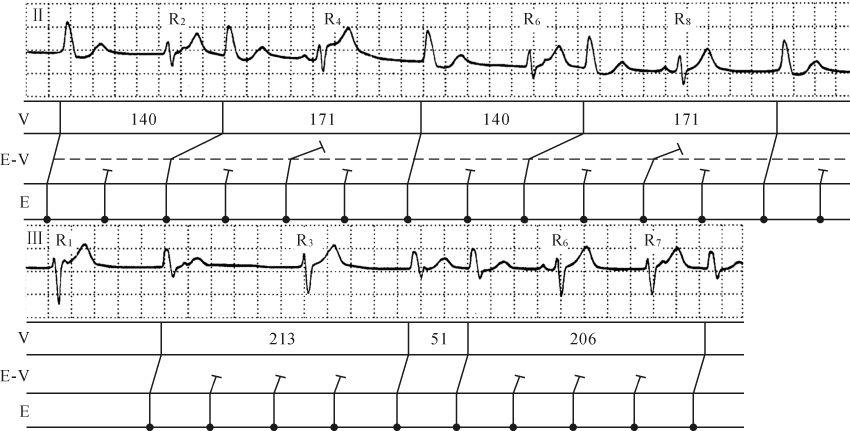
\includegraphics[width=5.73958in,height=2.90625in]{./images/Image00765.jpg}
 \captionsetup{justification=centering}
 \caption{例7 室性并行灶周围外出交替性A型文氏周期}
 \label{fig50-7}
  \end{figure} 

【精解与讨论】

室性并行灶周围外出交替性文氏周期的心电图特点为:①室性异位搏动的偶联间期不等;②EE间期由长→短→突长或由短→长→突长或短、长交替出现,周而复始;③由文氏周期推算出来的周期恰好为并行灶基本周期的2倍;④若并行灶周围近端2:1阻滞,远端文氏现象,出现连续3次并行灶激动受阻,则为A型交替性文氏周期;反之,近端文氏现象,远端2:1阻滞,出现连续2次并行灶激动受阻,则为B型交替性文氏周期,以A型多见。本例符合A型交替性文氏周期。但应与下列心律失常相鉴别:①室性早搏伴心室内双径路折返:本例室性异位搏动的偶联间期呈短、长两种,酷似室性早搏伴心室内双径路折返,但经慢径路折返引起长达0.92s的偶联间期则较罕见,结合Ⅲ导联两异位搏动之间能以成对出现的短E-E间期测得倍数关系,表明室性异位搏动系起源异常,而不是传导异常所致,可排除心室内双径路折返,偶联间期呈短、长两种,系室性并行灶发放激动的基本周期0.52s与窦性周期1.04s呈倍数关系所引起的偶然的巧合所致。②心室内有两个源起搏点:偶联间期短的异位搏动为折返型室性早搏,偶联间期长的则为加速的室性逸搏,此时异位搏动的QRS波形应该不一致,两异位搏动之间亦无倍数关系,而本例则刚好相反,故可以排除。

【心电图诊断】

①窦性心动过缓;②频发房室交接性逸搏或加速的房室交接性逸搏;③频发室性早搏或加速的室性逸搏,为室性并行心律伴并行灶周围外出交替性A型文氏周期或外出4:1传导;④不完全性干扰性房室分离。

例8 房室正道二、三度阻滞伴“获得性”预激综合征

【临床资料】

患者男性,64岁,临床诊断:冠心病、心房颤动。既往心电图未见预激综合征图形。

【心电图特征】

常规12导联(其中均V\textsubscript{3} ~V\textsubscript{6}
导联均为0.5mV)与长V\textsubscript{1}
导联系用洋地黄治疗后第8天同时记录,示窦性P波消失,代之以f波,QRS波形有3种:①宽大畸形,呈左束支阻滞型,时间0.18s,起始部似有δ波,于V\textsubscript{1}
、V\textsubscript{2} 导联呈rS型,V\textsubscript{5} 、V\textsubscript{6}
导联呈R型,其R-R间期绝对不规则;②呈正常形态,如长V\textsubscript{1}
导联R\textsubscript{2} 、R\textsubscript{3}
,其R-R间期固定为1.18s,频率51次/min;③形态介于上述两者之间,如长V\textsubscript{1}
导联R\textsubscript{9}
,其R-R间期为1.18s。停用洋地黄3天后记录Ⅰ导联,于心室率增快时出现宽大畸形QRS-T波群,于心室率减慢时出现正常QRS-T波群,当R-R间期0.97s时,出现介于两者之间的QRS-T波群,其前有明确的δ波,如R\textsubscript{6}
(A-V行中实线表示房室正道下传、虚线表示房室旁道下传、实线与虚线共同下传表示预激,V行中斜影部分表示预激程度)。

\begin{figure}[!htbp]
 \centering
 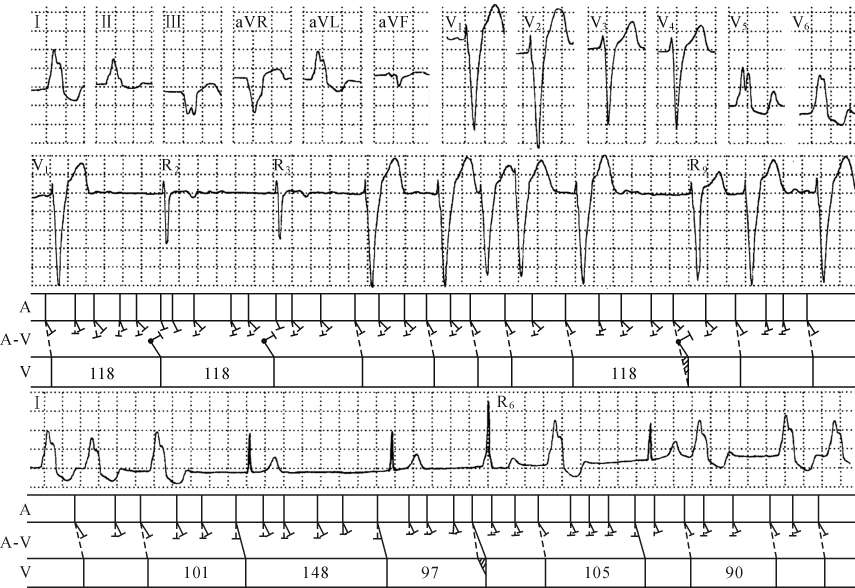
\includegraphics[width=5.78125in,height=3.96875in]{./images/Image00766.jpg}
 \captionsetup{justification=centering}
 \caption{例8 房室正道二、三度阻滞伴“获得性”预激综合征}
 \label{fig50-8}
  \end{figure} 

【精解与讨论】

本例常规十二导联及长V\textsubscript{1}
导联宽大畸形QRS-T波群时间宽达0.18s,形态酷似左束支阻滞型,有4种可能:①3相性左束支阻滞;②B型完全性预激综合征;③B型预激综合征合并3相性左束支阻滞;④心室内异位自律性增高型短阵性室性心动过速。结合Ⅰ导联R\textsubscript{6}
起始部有明确的δ波,R波无平顶挫折,应考虑这些宽大畸形QRS-T波群均由房室旁道下传的完全性预激波形,而排除3相性左束支阻滞。长V\textsubscript{1}
导联正常化QRS波群(R\textsubscript{2} 、R\textsubscript{3}
、R\textsubscript{9}
)有等长的周期,提示为房室交接性逸搏,其中R\textsubscript{9}
为f波由旁道下传与房室交接性逸搏经正道下传所产生的室性融合波,表明房室正道存在三度阻滞。

大部分房室旁道顺向传导的不应期极短≤0.35s,称为快旁道;小部分不应期相当长为0.60~3.0s,称为慢旁道,可有3相、4相阻滞及自律性。当慢旁道前传功能在在房室正道功能良好时未能显露,只有在正道出现阻滞后,旁道才显现出传导功能者称为“获得性”预激综合征。

本例长Ⅰ导联心室率增快时f波由旁道下传,而房室正道下传受阻,显示房室正道3相性阻滞;心室率减慢时f波由正道下传,而旁道下传受阻,显示房室旁道4相性阻滞。

【心电图诊断】

①心房颤动;②“获得性”完全性B型预激综合征;③三度房室传导阻滞;④房室交接性逸搏伴室性融合波;⑤停用洋地黄后表现为房室正道3相性阻滞、旁道4相性阻滞;⑥提示洋地黄中毒。

例9 房室结快径路隐匿性结-窦逆传致假性窦房传导阻滞或窦性停搏

【临床资料】

患者男性,32岁,临床诊断:病毒性心肌炎?

\begin{figure}[!htbp]
 \centering
 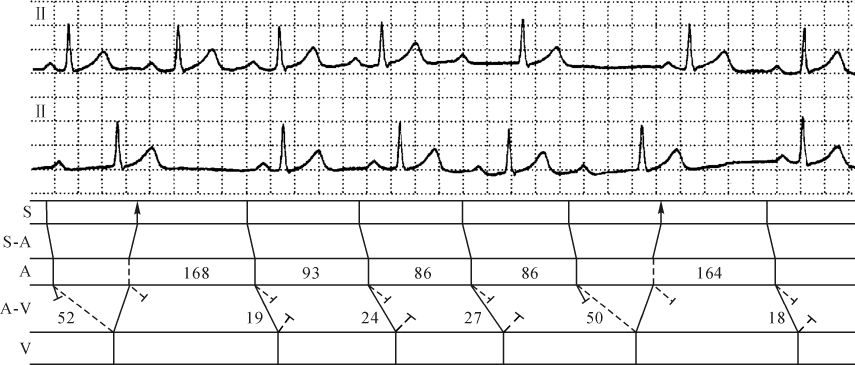
\includegraphics[width=5.78125in,height=2.45833in]{./images/Image00767.jpg}
 \captionsetup{justification=centering}
 \caption{例9 房室结快径路隐匿性结-窦逆传致假性窦房传导阻滞或窦性停搏}
 \label{fig50-9}
  \end{figure} 

【心电图特征】

Ⅱ导联连续记录,显示P-P间期0.82~0.93s,P-R间期分别由0.18s→连续3个0.25s→突然延长至0.52s或由0.18s→0.24s→突然延长至0.52s或由0.19s→0.24s→0.27s→突然延长至0.50s,其后出现长达1.68、1.64s的长P-P间期,与邻近的短P-P间期无倍数关系。食道心房调搏检查时用S\textsubscript{1}
-S\textsubscript{2} 法程控刺激,当S\textsubscript{1} -S\textsubscript{2}
为290ms时,其S\textsubscript{2} -R间期为280ms,当S\textsubscript{1}
-S\textsubscript{2} 为280ms时,其S\textsubscript{2}
-R间期为500ms,S-R间期呈跳跃式延长。

【精解与讨论】

本例P-P间期基本规则,而P-R间期却成倍增加,符合房室结内双径路传导;此外,快径路P-R间期由0.18s增至0.24~0.25s,其递增量≥0.06s,该房室传导时间改变有2种解释:①快径路内不典型的文氏现象,最短的P-R间期系长P-P间期后快径路得到充分休息所致;②房室结内存在三径路传导,即最短的P-R间期属快径路,次长的P-R间期为中速径路,最长的P-R间期则为慢径路传导。经食道调搏检测,房室传导曲线仅有一处中断现象,表明房室结内仅存在双径路传导。

值得注意的是本例长P-R间期之后均出现长P-P间期,有3种解释:①窦性激动由房室结慢径路下传心室,同时又循快径路隐匿性逆传至窦房交接区与窦性激动相互干扰形成假性二度窦房传导阻滞或逆传至窦房结使其节律重整引起假性窦性停搏。既然由快径路逆传的激动通过心房至窦房交接区或窦房结,为何未使心房肌除极产生逆行P\textsuperscript{-}
波呢?可能类似高钾血症引起的窦-室传导,经快径路逆传的激动优先通过结间束逆传到窦房交接区或窦房结,并未进入心房肌,故未能使心房肌除极而产生逆行P\textsuperscript{-}
波(梯形图中A行以虚线表示)或逆行P\textsuperscript{-}
波与窦性P波在心房内相融合而表现为等电位线。②可能存在真正的二度窦房传导阻滞或窦性停搏,但均发生在长P-R间期之后,似乎太巧合。③窦性P波重叠在T波上,但T波形态光滑,不支持有P波重叠。以第1种解释较为合理。

【心电图诊断】

①窦性心律;②房室结内双径路传导,其中快径路呈3:2~5:4传导的不典型文氏现象,慢径路为二度~高度阻滞呈3:1~5:1传导;③房室结快径路隐匿性结-窦逆传致假性窦房传导阻滞或窦性停搏;④房室结慢径路内蝉联现象。

例10 双结病合并房室结内双向性三径路传导

【临床资料】

患者女性,35岁,近1周晕厥数次。临床诊断:晕厥原因待查,病毒性心肌炎?

\begin{figure}[!htbp]
 \centering
 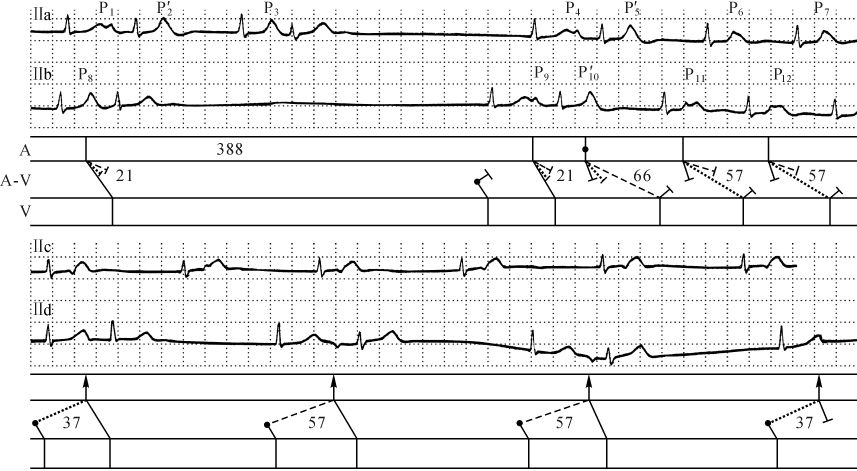
\includegraphics[width=5.79167in,height=3.17708in]{./images/Image00768.jpg}
 \captionsetup{justification=centering}
 \caption{例10 双结病合并房室结内双向性三径路传导}
 \label{fig50-10}
  \end{figure} 

【心电图特征】

Ⅱa、Ⅱb导联连续记录,窦性的基本P-P间期0.76~0.79s,心率76~79次/min,Ⅱa导联长P-P间期2.68s,与短P-P间期无倍数关系,Ⅱb导联长P-P间期3.88s,为短P-P间期的5倍,期间可见缓慢的房室交接性逸搏出现;P′\textsubscript{2}
、P′\textsubscript{5} 、P′\textsubscript{10}
提早出现,落在T波顶峰上,下传的P′-R间期0.66~0.69s,偶联间期相等,代偿间歇不完全,为房性早搏经房室结慢径路下传(梯形图A-V行中以长条虚线表示);P\textsubscript{1}
、P\textsubscript{3} 、P\textsubscript{4} 、P\textsubscript{8}
、P\textsubscript{9}
落在T波降肢或顶峰上,下传的P-R间期0.21s,由快径路下传(以实线表示);P\textsubscript{6}
、P\textsubscript{7} 、P\textsubscript{11} 、P\textsubscript{12}
落在T波顶峰或上升肢上,下传的P-R间期0.57s,循中速径路下传(以圆点虚线表示)。Ⅱc、Ⅱd导联均未见窦性P波,Ⅱc导联R-R间期1.19~1.25s,频率48~50次/min,QRS波群后面均跟随逆行P\textsuperscript{-}
波,R-P\textsuperscript{-}
间期0.21s,系房室交接性逸搏经快径路逆传至心房。Ⅱd导联重复出现QRS-P\textsuperscript{-}
-QRS或QRS-P\textsuperscript{-}
序列,表现为房室交接性逸搏及其反复搏动,逸搏QRS波形与反复搏动的QRS波形略异,为非时相性心室内差异性传导,逸搏周期1.46~1.53s,频率39~41次/min,R-P\textsuperscript{-}
间期0.37s、0.51s呈短、长两种,分别由中速径路、慢径路逆传,显示房室结内逆向性三径路传导。

【精解与讨论】

本例出现窦性停搏、窦房传导阻滞、缓慢而不规则的房室交接性逸搏、短暂性全心停搏,符合双结病的心电图诊断条件。电生理研究表明,房室传导曲线有两处中断现象,每一处中断的时距≥0.06s,即提示房室结内存在三径路传导。房性早搏或窦性激动落在T波上下传的P-R间期出现长、短数种,有3种可能:①干扰性P-R间期延长,此时P-R间期长、短不一,其R-P间期与P-R间期呈反比关系,即R-P间期短,其P-R间期长;反之,R-P间期长,其P-R间期短。②房室结内多径路传导,此时不同径路下传的P-R间期各自固定,R-P间期与P-R间期不呈反比关系。③上述两者兼有之,此时同一径路下传的P-R间期可略有长短,但应<0.06s。本例房性早搏的P′波落在T波顶峰上,其下传的P′-R间期0.66~0.69s,而窦性P波落在T波上升肢上,其P-R间期却为0.21s、0.57s,存在着R-P间期与P-R间期不呈反比关系的矛盾现象,很难以干扰性P′-R间期延长来解释,应考虑房性早搏由慢径路下传,窦性激动由快径路、中速径路下传,即房室结内存在顺向性三径路传导。Ⅱc、Ⅱd导联房室交接性逸搏出现不完全及完全性反复搏动,其R-P\textsuperscript{-}
间期有0.21s、0.37s、0.57s三种,无论其P\textsuperscript{-}
波形态是否一致,均符合房室结内逆向性三径路传导。

【心电图诊断】

①窦性心律;②窦性停搏;③高度窦房传导阻滞;④频发房性早搏;⑤房室结内双向性三径路传导;⑥缓慢而不规则的房室交接性逸搏伴停搏;⑦双结病、短暂性全心停搏。

例11 室性早搏二联律伴心室折返径路内双径路传导

【临床资料】

患者女性,49岁,临床诊断:冠心病?

\begin{figure}[!htbp]
 \centering
 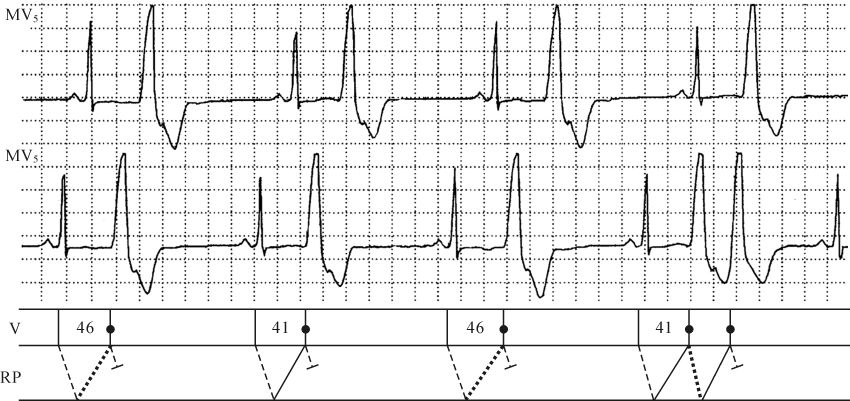
\includegraphics[width=5.73958in,height=2.70833in]{./images/Image00769.jpg}
 \captionsetup{justification=centering}
 \caption{例11 室性早搏二联律伴心室折返径路内双径路传导}
 \label{fig50-11}
  \end{figure} 

【心电图特征】

DCG示室性早搏13498次、成对室性早搏179次、短阵性室性心动过速31次。MV\textsubscript{5}
导联连续记录,示窦性搏动的T波振幅低平,室性早搏二联律,偶呈成对出现,其QRS波形一致,偶联间期为0.46s、0.41s交替出现,符合心室折返径路内双径路传导(RP行长条虚线表示进入心室折返径路前的心室内传导,实线、短粗虚线分别表示快、慢径路传导)。

【精解与讨论】

(1)心室折返径路内双径路传导的基本概念:有狭义和广义之分。前者指主导节律(多为窦性)的激动在心室内折返过程中,传出支因存在纵向分离而形成快、慢双径路,其折返出口只有一个,出现偶联间期短、长两种和QRS波形一致的室性早搏;而后者系传出支因心室内特殊传导纤维参与,充当并构成两条不同的传导径路和出口,出现偶联间期固定、QRS波形两种或偶联间期长、短两种和QRS波形两种的室性早搏。

(2)心室折返径路内双径路传导的6种心电图表现及其机制:①室性早搏偶联间期长、短交替型:本例室性早搏二联律,偶联间期呈长、短交替出现,QRS波形一致,与1983年Kinoshita等首先报道1例相同,提示折返径路内纵向分离为快、慢双径路,其出口相同。当第1个窦性冲动进入心室内折返径路经慢径路传导形成0.46s偶联间期,而第2个窦性冲动进入折返径路时,慢径路尚处于有效不应期,冲动只能沿快径路传导形成0.41s偶联间期,如此周而复始便形成偶联间期长、短交替出现;或者两条长、短不同的折返径路的传出支有一个公共出口,类似房室结Y型双径路,也可出现长、短两种偶联间期。②偶联间期无规律交替型:室性早搏QRS波形一致,偶联间期呈长-长-短-短、短-长-长或长-短-短等无规律交替,无中间状态,与窦性周期的长短无关。③长、短偶联间期分别连续出现≥3次,且相互突然转变,表现为快、慢径路内蝉联现象。④成对室性早搏型:在适当长或短的偶联间期时,室性早搏呈成对出现,QRS波形相似,其R′-R′间期较短,易出现Ron-T现象而诱发严重的室性心律失常。1979年Kinoshita等报道的成对早搏发生在较长的偶联间期后,认为心室折返径路内存在纵向分离和超常传导是引起成对室性早搏的原因,即窦性冲动进入心室内折返径路沿慢径路传至心室引起第1个早搏,其逆传快径路的冲动折回慢径路时恰好遇及此超常期才再次由慢径路传入心室形成第2个早搏,否则,该冲动落在超常期偏前或偏后均会受阻。本例成对早搏、短阵性室性心动过速多发生在较短的偶联周期后,其折返方式是先由快径路传出产生第1个早搏,后又经慢径路缓慢折回,使快径路有充分的时间脱离不应期或遇及快径路的超常期,使得冲动能再沿快径路传出形成第2、3个早搏,这第2、3个早搏属双径路之间的折返所致,故第2个折返性早搏的出现是折返径路内存在双径路传导的又一重要佐证。⑤偶联间期固定而R′波两种形态交替型:常称为双形性室性早搏,系传出支有两条传导径路和两个出口,但传至心室所需时间是相等的,类似房室结内倒Y型双径路。⑥偶联间期长、短两种及R′波两种形态交替型:常称为双源性室性早搏,系传出支有两条传导径路和两个出口,且传至心室所需时间是不等的。

(3)鉴别诊断:①室性早搏折返径路内交替型文氏周期:折返径路内双径路传导其偶联间期由短变长或由长变短,不经过折返中断就变短或变长,仍保持显性二联律或三联律;而折返径路内交替性文氏周期需经过一次折返中断后偶联间期才变短或变长,出现隐性二联律或偶数变异性隐性二联律,但有时两者可并存于同一病例。②室性并行心律:折返径路内双径路传导其偶联间期为固定的长、短两种,两异位搏动之间无倍数关系,与属起源异常的并行心律的偶联间期长短不一及两异位搏动之间有倍数关系迥然不同。③多源性室性早搏:属起源异常,系心室内有多个异位起搏点发放冲动引起偶联间期长短不一、QRS波形多变,有时与本文第6型心室内双径路折返性早搏较难鉴别,但后者偶联间期长、短两种始终是固定的可资鉴别。

【心电图诊断】

①窦性心律;②频发室性早搏二联律,有时呈成对出现;③心室折返径路内双径路传导。

例12 加速的房性、房室交接性逸搏心律伴传导系统多水平阻滞

【临床资料】

患者男性,17岁,临床诊断:先天性心脏病、原发孔型房间隔缺损合并二尖瓣裂。

【心电图特征】

心脏手术前常规心电图示窦性P波频率65次/min,Ⅱ、V\textsubscript{2}
导联P波形态高尖,电压分别为0.3mV、0.45mV,时间0.10s,V\textsubscript{1}
Ptf值为-0.12mm·s;P-R间期0.23s;QRS波群时间0.12s,Ⅰ导联呈qRS型,Ⅲ导联呈rSr′型,电轴-30°,aVR导联呈qR型,q/R<1,V\textsubscript{1}
导联呈rsR′s′型,R′/s′>1,V\textsubscript{5}
导联呈Rs型,R\textsubscript{V\textsubscript{1}}
+S\textsubscript{V\textsubscript{5}}
=2.1mV;aVL导联T波低平,V\textsubscript{6} 导联T波浅倒。

长Ⅱ导联系术后第1天描记,P波呈负、正双相,时间0.15s,其中正相波呈双峰切迹,两峰距0.06s,与术前Ⅱ导联及术后第8天恢复窦性节律时Ⅱ导联P波形态均有明显差异,P-P间期0.54s,频率111次/min;QRS波群呈rS型,S波错折,时间0.12s,电轴增至-59°,与术前QRS波形不一致,R-R间期由0.56s→0.63s→0.97s逐渐延长或由0.56s→1.06s逐渐延长,呈交替出现。

\begin{figure}[!htbp]
 \centering
 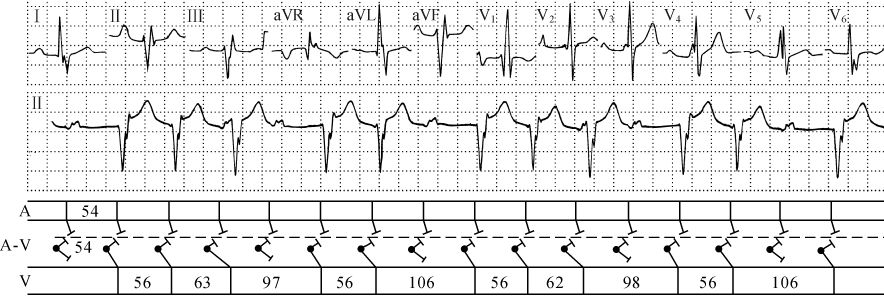
\includegraphics[width=5.96875in,height=2.02083in]{./images/Image00770.jpg}
 \captionsetup{justification=centering}
 \caption{例12 加速的房性、房室交接性逸搏心律伴传导系统多水平阻滞}
 \label{fig50-12}
  \end{figure} 

【精解与讨论】

心电轴左偏是判断原发孔型房间隔缺损重要依据之一。本例心电轴左偏,Ⅱ、V\textsubscript{2}
导联P波高尖类似“肺型P波”,V\textsubscript{1}
Ptf值明显增大,V\textsubscript{1}
导联QRS波群以R波为主,表明存在右心房、右心室肥大及左心房负荷过重,符合原发孔型房间隔缺损的病理生理改变。

本例重点分析长Ⅱ导联心律失常,长Ⅱ导联P波呈负、正双相,其中正相波呈双峰切迹,两峰距0.06s,P波时间达0.15s,与术前Ⅱ导联及术后第8天恢复窦性节律时Ⅱ导联P波形态均有明显差异,考虑该P波激动起源于心房,并提示存在不完全性心房内传导阻滞,频率111次/min,为加速的房性逸搏心律。QRS波形与术前不一致,电轴增至-59°,R-R间期由0.56s→0.63s→0.97s逐渐延长或由0.56s→1.06s逐渐延长,呈交替出现,呈现4:3~3:2不典型文氏现象,其基本周期为(0.56+0.63+0.97)÷4=0.54s或(0.56+1.06)÷3=0.54s,恰好与P-P间期一致,P-R间期明显延长(最短的为0.54s,最长的达0.66s),考虑P波与QRS波群无关,存在等频性完全性房室分离,可能由三度房室传导阻滞或生理性干扰引起的假性三度房室传导阻滞所致。该QRS波群起源部位有2种可能:①起源于高位室间隔:所发放的激动表现为加速的室性逸搏心律伴异-肌交接区外出3:2~4:3不典型文氏现象;②起源于房室交接区:表现为加速的房室交接性逸搏心律伴结-室3:2~4:3不典型文氏现象及左前分支阻滞。

心房与高位室间隔或房室交接区两个节律点频率相等,可能是偶然巧合,但更可能是一种特殊的电生理影响------“同步化”或“趋同”现象所致。Segers认为两个节律点频率相差<25\%时,易出现“同步化”或“趋同”现象,即慢的频率逐渐增速,接近于快的频率直至相等,形成等频率搏动。

【心电图诊断】

术前常规心电图:①窦性心律;②右心房、右心室肥大;③V\textsubscript{1}
Ptf值明显增大,提示左心房负荷过重;④一度房室传导阻滞;⑤不定型心室内传导阻滞;⑥侧壁T波改变。

长Ⅱ导联心电图:①加速的房性逸搏心律;②不完全性心房内传导阻滞;③完全性房室分离,可能由三度房室传导阻滞或生理性干扰引起的假性三度房室传导阻滞所致;④加速的高位室性逸搏心律伴异-肌交接区3:2~4:3不典型文氏现象或加速的房室交接性逸搏心律伴结-室3:2~4:3不典型文氏现象及左前分支阻滞;⑤不定型心室内传导阻滞。

例13 右心房内文氏现象合并间歇性左心房内传导阻滞

【临床资料】

患者男性,68岁,临床诊断:冠心病、病窦综合征?

\begin{figure}[!htbp]
 \centering
 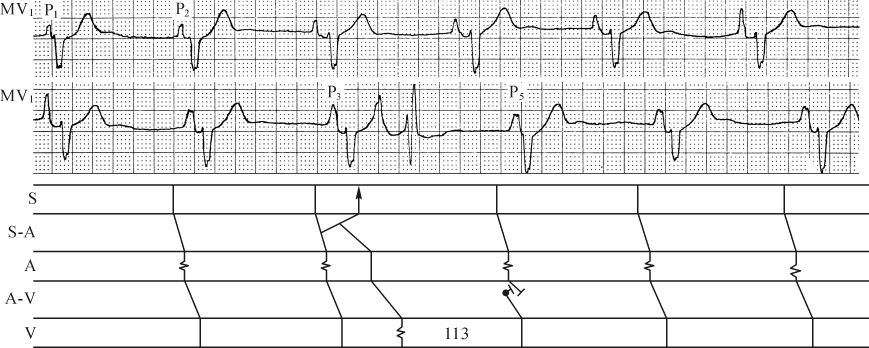
\includegraphics[width=5.875in,height=2.34375in]{./images/Image00771.jpg}
 \captionsetup{justification=centering}
 \caption{例13 右心房内文氏现象合并间歇性左心房内传导阻滞}
 \label{fig50-13}
  \end{figure} 

【心电图特征】

MV\textsubscript{1}
导联连续记录,显示窦性P-P间期1.30~1.41s,频率43~46次/min,P波形态多变,上行P波形态尖而窄,振幅分别由0.25→0.30→0.30→0.35→0.35→0.62mV逐渐增高,P波时间0.06~0.08s;下行P波形态由尖而窄变成高而宽,前3个P波振幅由0.60→0.41→0.50mV,时间由0.08→0.12(呈双峰切迹,两峰距0.04s)→0.11s,后3个P波形态基本一致,振幅0.4mV,时间0.12s,呈双峰切迹,两峰距0.04s;下行第4个P波提早出现重叠于T波上,其形态尖耸,下传的PR间期延长、QRS波群呈右束支阻滞型,其后代偿间歇1.33s小于下行窦性P-P间期而呈次等周期代偿;大部分P-R间期0.16s,而上行P\textsubscript{1}
-R间期0.07s,P\textsubscript{2} -R间期0.11s,下行P\textsubscript{5}
-R间期0.12s均较基本P-R间期缩短,这3个搏动的P波与QRS波群显然无关,为房室交接性逸搏。

【精解与讨论】

(1)诊断心房内文氏现象的前提是P-P间期规则,以排除频率依赖性心房内传导阻滞、房性融合波及游走节律或房性异位搏动。本例上行前半部分P-P频率46次/min,后半部分及下行P-P规则,频率43次/min,虽然P-P略有互差,但P波形态、振幅由低窄向尖耸有规律地演变,表明窦性激动在右心房内传导速度逐渐减慢,符合右心房内文氏现象。下行在P-P间期规则时,P波出现3种形态:高而窄、高而宽及介于两者之间(如下行P\textsubscript{3}
),前者显然为单纯性右心房内传导阻滞所致,后两者除右心房内传导阻滞外尚合并左心房内传导阻滞,出现类似双心房肥大的巨大型P波。

(2)窦房交接性早搏的P′波形态与窦性P波可一致或略异,这取决于该早搏激动下传途径与窦性P波是否一致、心房除极顺序有无改变。其后代偿间歇在P-P间期规则时,可呈等周期、次等周期或不完全代偿间歇,这取决于窦房交接性早搏的冲动逆传重整窦性节律所需时间与前向传导激动心房所需时间差值的多少。当逆传重整窦性节律先于前传激动心房,且两者时间差刚好为窦房传导时间,则表现为等周期代偿,与窦性早搏难以鉴别;当逆传重整窦性节律明显先于前传激动心房,则呈次等周期代偿;反之,则表现为不完全代偿间歇与房性早搏难以鉴别。

(3)下行第5个搏动为房室交接性逸搏,其逸搏周期为1.13s,较R\textsubscript{1}
-R\textsubscript{2}
逸搏周期1.32s短。一般说来,逸搏周期多较恒定,而本例该逸搏周期为何突然缩短?有3种解释:①该逸搏点位置较高,窦房交接性早搏在下传中较早地使其节律重整,加上该早搏P′-R间期干扰性延长使QRS波群后延;②窦房交接性早搏在下传中促进房室交接性逸搏提早发放;③逸搏起搏点节律不规则。以第1种可能性为大。

【心电图诊断】

①窦性心动过缓;②一过性右心房内文氏现象;③不完全性右心房内传导阻滞合并间歇性左心房内传导阻滞;④窦房交接性早搏伴干扰性P′-R间期延长及心室内差异传导;⑤房室交接性逸搏。

例14 左心房肥大合并3相性右心房内传导阻滞

【临床资料】

患者男性,21岁,临床诊断:风湿性心脏病、二尖瓣狭窄伴关闭不全、心力衰竭。

\begin{figure}[!htbp]
 \centering
 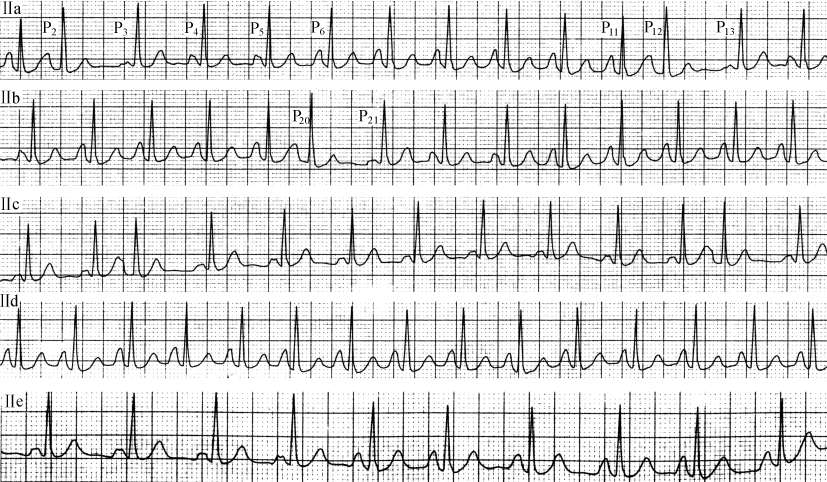
\includegraphics[width=5.58333in,height=3.25in]{./images/Image00772.jpg}
 \captionsetup{justification=centering}
 \caption{例14 左心房肥大合并3相性右心房内传导阻滞}
 \label{fig50-14}
  \end{figure} 

【心电图特征】

Ⅱa、b连续记录,窦性P-P间期0.54~0.66s,频率91~111次/min,P波形态有4种:①P\textsubscript{2}
、P\textsubscript{12} 、P\textsubscript{20}
提早出现重叠于T波上,偶联间期相等,为房性早搏;②房性早搏后第1个窦性P波(P\textsubscript{3}
、P\textsubscript{13} 、P\textsubscript{21}
)时间0.10s,呈双峰切迹,第2峰高于第1峰,两峰距0.06s,属“二尖瓣型P波”,可能伴有心房内差异性传导;③P\textsubscript{1}
、P\textsubscript{6} ~P\textsubscript{11}
形态尖耸,电压0.35~0.40mV,时间0.10~0.11s,为“肺型P波”,发生在频率较快时(105~111次/min),符合3相性右心房内传导阻滞;④房性早搏后第2、3个窦性P波(如P\textsubscript{4}
、P\textsubscript{5} )形态一致,介于P\textsubscript{3}
与P\textsubscript{6}
之间,时间0.10~0.11s,电压0.20~0.22mV,发生在频率稍快时(91~103次/min),可能系右心房内3相传导阻滞程度较轻所致。Ⅱc系静卧10min后记录,P-P间期0.60~0.72s,频率83~100次/min,P波时间0.10~0.11s,呈双峰切迹,两峰距0.04s,为“二尖瓣型P波”,房性早搏后第1个P波较其他P波宽0.02s。Ⅱd系起卧活动数次后记录,P-P间期0.53~0.58s,频率104~113次/min,P波形态尖耸,电压0.35~0.40mV,时间0.10~0.11s,属“肺型P波”。Ⅱe系Ⅱd记录后静卧数分钟后记录,P-P间期0.60~0.69s,出现“二尖瓣型P波”和“肺型P波”(电压0.32~0.35mV),符合左心房肥大伴间歇性不完全性右心房内传导阻滞。

【精解与讨论】

本例患者经超声心动图、心脏三位片检查及手术(二尖瓣置换术)证实为左心房、左心室肥大,而右心房、右心室无明显增大。上述心电图出现“肺型P波”显然不能用右心房肥大或右心房负荷过重来解释,尤其是Ⅱe“二尖瓣型P波”的P-P间期与“肺型P波”的P-P间期均不固定,而两者相互转变时其P-P间期却规则,表明右心房内传导组织不应期出现病理性延长,呈现间歇性右心房内传导阻滞,难以用游走节律、房性异位节律及房性融合波解释。心率减慢时,如Ⅱc及Ⅱa、b房性早搏后的第1个P波均为“二尖瓣型P波”,而心率增快时(>105次/min),如Ⅱd及Ⅱa、b出现“肺型P波”,且比Ⅱe的“肺型P波”高而宽,说明窦性激动在右心房内发生较严重的3相阻滞,导致右心房除极延迟至左心房除极结束之后出现高而宽的P波,但应与下列心律失常相鉴别:

(1)房性早搏后窦房结内或心房内游走节律:房性早搏逆传侵入窦房结,使原来窦性起搏点暂时受到抑制,窦房结其他部位或心房内异位起搏点取而代之,此时的P-P间期互差>0.16s,P波形态、振幅渐变和多变,P-R间期不恒定。本例房性早搏后P波不符合渐变、多变特点,结合临床、Ⅱc图形,可排除游走节律。

(2)房性早搏后伴心房内差异性传导:心房内传导系统的结间束与上房间束不应期是不一致的,房性早搏在心房内传导系统可发生隐匿性传导产生一次新的不应期,使其后窦性激动的心房除极顺序发生改变引起窦性P波畸形,通常仅影响早搏后第1个窦性P波,少数可影响数个窦性P波。本例房性早搏后第1~3个窦性P波形态与Ⅱc窦性P波不一致,可用心房内差异性传导解释,但以后众多的“肺型P波”实难以此解释。

(3)早搏后非阵发性房性心动过速:房性早搏逆传可暂时抑制窦房结发放激动,诱发心房内异位起搏点激动发放。本例房性早搏后虽然P波频率逐渐加快直至固定,符合“起步现象”;房性早搏后第2、3个P波亦可用房性融合波来解释,但结合Ⅱc、Ⅱd图形,早搏后非阵发性房性心动过速可能性很少。

(4)左心房内4相性阻滞:其特点为心率增快时窦性P波正常或“肺型P波”(右心房肥大时),而心率减慢时出现“二尖瓣型P波”,且“二尖瓣型P波”时间大于“肺型P波”时间。而本例“肺型P波”时间≥“二尖瓣型P波”时间,且临床上证实左心房肥大而无右心房肥大,显然不符合左心房内4相性阻滞。

(5)右心房内文氏现象:Ⅱa、b导联P波形态由低平切迹→“肺型P波”有规律地改变,酷似文氏型右心房内传导阻滞,但因其P-P间期略有不规则,结合Ⅱe、d优先考虑3相性右心房内传导阻滞。

【心电图诊断】

①窦性心律;②左心房肥大合并间歇性不完全性右心房内传导阻滞;③频发房性早搏伴早搏后心房内差异性传导;④3相性右心房内传导阻滞。

例15 高钾血症引起窦-室传导、窦-室文氏现象及心电阶梯现象

【临床资料】

患者女性,43岁,临床诊断:慢性肾炎,高钾血症(血钾7.2mmol/L)。

【心电图特征】

常规心电图示P波消失,QRS波群增宽,时间0.14s;Ⅰ、aVL呈rS型,S\textsubscript{aVL}
>S\textsubscript{Ⅰ}
,Ⅱ导联呈Rs型,Ⅲ导联呈qR型,aVF导联呈R型,R\textsubscript{Ⅲ}
>R\textsubscript{Ⅱ} ,电轴由入院时+51°增至+108°,V\textsubscript{5}
导联S波加深,应考虑左后分支传导阻滞;V\textsubscript{2}
~V\textsubscript{6}
导联T波尖耸,两肢对称,基底部变窄呈“帐篷状”,符合高钾血症的心电图改变。长V\textsubscript{1}
导联R-R间期由0.81~0.86s→0.68~0.70s→1.51~1.59s,呈顿挫型5:4传导文氏现象,S波的振幅由深→浅→稍深,T波由直立→负、正双相→低平,随文氏周期交替性改变,每一组文氏周期的末次搏动的S、T波振幅均介于其前后两个QRS、T波振幅之间。经腹膜透析等处理,血钾和心电图均恢复正常。

【精解与讨论】

(1)房室文氏现象的心电图特征:①P-R间期逐渐延长,直至P波受阻QRS波群脱落;②P-R间期延长的增量逐渐减少;③R-R间期逐渐缩短,直至出现较长的R-R间期,呈“渐短突长”规律;④长间歇后的第1个R-R间期大于间歇前的一个R-R间期;⑤长R-R间期小于任何两个短R-R间期之和;⑥长R-R间期后的第1个心搏的P-R间期恢复正常。本例2个完整的文氏周期中,其长R-R间期均大于两个短R-R间期之和,故为顿挫型5:4文氏现象,而不是4:3传导的文氏现象,即窦性基本周期为0.60~0.63s(86+70+159/5=0.63、81+68+151/5=0.60),第4个搏动发生隐匿性传导,第5个搏动出现真正的阻滞。

\begin{figure}[!htbp]
 \centering
 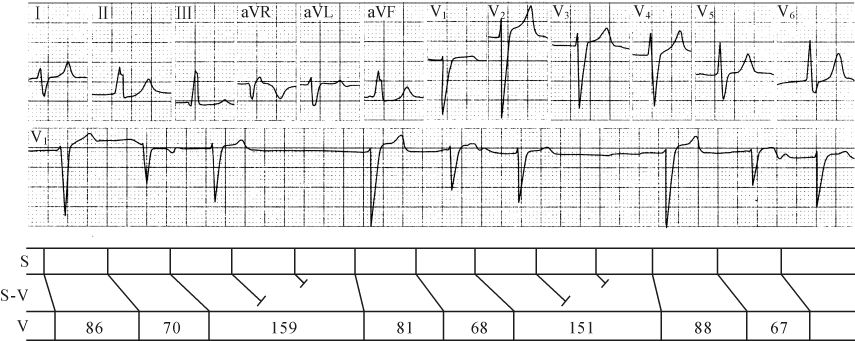
\includegraphics[width=5.78125in,height=2.30208in]{./images/Image00773.jpg}
 \captionsetup{justification=centering}
 \caption{例15 高钾血症引起窦-室传导、窦-室文氏现象及心电阶梯现象}
 \label{fig50-15}
  \end{figure} 

(2)心电阶梯现象的心电图特征:①心搏来源恒一,多为窦性(本例为窦-室传导);②QRS波群时间固定不变,仅QRS波群的振幅如R波由低→高或由高→低、S波由浅→深或由深→浅呈渐变的周期性改变,可同时伴有ST段、T波形态与振幅周期性改变;③常为一过性出现;④与心外因素无关,如呼吸、体位、胸腔积液等。心电阶梯现象发生机制可能是部分心室肌不应期明显延长或膜电位水平出现周期性高低改变所致,它的出现可提示心肌有广泛的严重病变,其预后则与原发病有关。

(3)本例系高钾血症患者,常规十二导联及长V\textsubscript{1}
导联均未见P波,QRS波群增宽,T波高尖呈“帐篷状”,应考虑窦-室传导。长V\textsubscript{1}
导联R-R间期由长→短→突长,符合文氏现象特点,因心房肌麻痹,未见P波,该文氏现象发生部位可能在窦房交接区、房室结或希氏束,明确部位有一定困难。长V\textsubscript{1}
导联QRS波群的S波、ST段、T波的形态与振幅随文氏周期呈渐变的周期性改变,符合心电阶梯现象。

【心电图诊断】

①窦-室传导;②左后分支传导阻滞;③不定型心室内传导阻滞;④窦房交接区、房室交接区或希氏束内顿挫型5:4文氏现象;⑤心电阶梯现象;⑥心电图改变符合高钾血症。

例16 房室交接性早搏诱发窦性回波

【临床资料】

患者女性,82岁,临床诊断:冠心病、糖尿病。

【心电图特征】

Ⅱ、V\textsubscript{5}
导联同步记录,示窦性P-P间期0.83~0.84s,P-R间期0.15s,下传的QRS波群呈完全性右束支阻滞型;第3个搏动系提早出现P\textsuperscript{-}
-QRS-T波群,P\textsuperscript{-}
-R间期0.09~0.10s;第4个搏动系提早出现,其P-QRS-T波群的形态与窦性一致,P\textsubscript{2}
-P\textsubscript{4} 间期1.05s大于窦性P-P间期,P\textsubscript{4}
-P\textsubscript{5} 间期0.86s,略长于窦性P-P间期,P\textsubscript{2}
-P\textsubscript{5} 间期>2个窦性P-P间期。

\begin{figure}[!htbp]
 \centering
 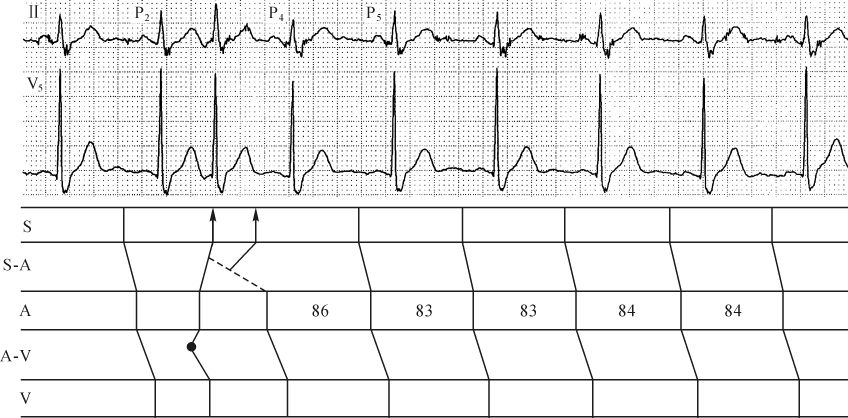
\includegraphics[width=5.72917in,height=2.82292in]{./images/Image00774.jpg}
 \captionsetup{justification=centering}
 \caption{例16 房室交接性早搏诱发窦性回波}
 \label{fig50-16}
  \end{figure} 

【精解与讨论】

本例第3个搏动提早出现的P′波为逆行P\textsuperscript{-}
波,其P\textsuperscript{-}
-R间期<0.12s,为房室交接性早搏;值得注意的是第4个搏动,其P波形态与窦性P波一致,有3种可能:①是真正的窦房结所发放的激动,第3个搏动为间位型房室交接性早搏:P\textsubscript{2}
-P\textsubscript{4}
间期大于窦性P-P间期,可考虑第4个搏动在下传心房过程中遇及房室交接性早搏逆传窦房交接区时所产生的不应期而出现干扰性窦房传导延缓使P\textsubscript{4}
后延,但P\textsubscript{2} -P\textsubscript{5}
间期应等于2个窦性P-P间期,可本例却>2个窦性P-P间期,表明房室交接性早搏的冲动已逆传至窦房结使其节律重整,故此种可能性可予以排除。②房室交接性早搏的冲动逆传窦房结促使其冲动提前发放:一般地说,异位冲动逆传窦房结使其节律重整,下一个窦性冲动的形成往往是后延的,而出现不完全性代偿间歇。③房室交接性早搏诱发窦性回波:异位冲动逆传窦房结时,在窦房交接区沿着另一条径路折回心房,形成窦性回波,该P波形态与窦性P波是否一致,主要取决于该折返激动下传途径、心房除极顺序与窦性激动是否一致及心房有无脱离不应期有关。至于P\textsubscript{4}
-P\textsubscript{5}
间期的长短则取决于该折返激动前向传导除极心房所需时间与逆向传导重整窦房结节律所需时间的差值,若先逆传重整窦房结节律,后前传除极心房且两者所需时间的差值刚好为窦房传导时间,则P\textsubscript{4}
-P\textsubscript{5}
间期刚好等于1个窦性P-P间期;若先前传心房产生P波,后逆传重整窦房结节律,则P\textsubscript{4}
-P\textsubscript{5}
间期>1个窦性P-P间期;反之,若先逆传重整窦房结节律,后前传心房产生P波,则P\textsubscript{4}
-P\textsubscript{5} 间期<1个窦性P-P间期。本例以第③种可能性为大。

【心电图诊断】

①窦性心律;②房室交接性早搏诱发窦性回波;③完全性右束支阻滞。

例17 心房颤动合并几乎完全性房室传导阻滞及韦金斯基现象

【临床资料】

患者男性,74岁,临床诊断:冠心病、洋地黄中毒。

【心电图特征】

Ⅱ导联连续记录,窦性P波消失,代之以f波,大多数R-R间期2.34~2.60s,频率23~26次/min,QRS波形、时间正常;第3个搏动为提早出现的宽大畸形QRS-T波群,偶联间期1.0s,其后连续出现2次形态、时间均正常的QRS波群,其R-R间期不规则;T波倒置。

\begin{figure}[!htbp]
 \centering
 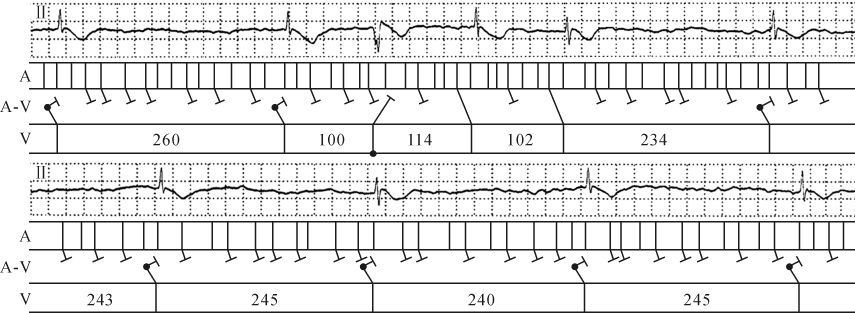
\includegraphics[width=5.78125in,height=2.11458in]{./images/Image00775.jpg}
 \captionsetup{justification=centering}
 \caption{例17 心房颤动合并几乎完全性房室传导阻滞及韦金斯基现象}
 \label{fig50-17}
  \end{figure} 

【精解与讨论】

本例基本节律为心房颤动,大多数R-R间期缓慢而略不规则,频率23~26次/min,QRS波形呈室上性,提示这些QRS波群不是由f波下传,而是由房室交接性逸搏起搏点被动地发放冲动,其频率缓慢而不规则,提示下级起搏点功能欠佳;为何f波不能下传心室?考虑过量的洋地黄抑制了房室交接区的传导以致出现三度房室传导阻滞。值得注意的是,室性异位搏动后连续出现了2次由f波下传的QRS波群,考虑房室交接区阻滞区的远端受到室性异位搏动强刺激后,使阻滞区应激阈值降低,原不能通过阻滞区的f波却能意外地下传心室,形成韦金斯基易化作用,属对侧促进传导;易化作用后下传的激动本身又作为强刺激,使阻滞区应激阈值又暂时降低,致适时而来的f波能再次下传,形成韦金斯基效应,为同侧促进传导。该室性异位搏动的频率为60次/min,属加速的室性逸搏,但与基本的R-R间期相比,则又明显地提早出现,故可考虑为室性早搏。

韦金斯基现象仅见于有传导阻滞的器质性心脏病,它的出现一方面表示传导系统有病变,另一方面与逸搏一样是免遭心室停搏的保护性反应。

【心电图诊断】

①心房颤动伴极缓慢的心室率;②缓慢的房室交接性逸搏心律伴不齐;③几乎完全性房室传导阻滞;④室性异位搏动诱发房室交接区韦金斯基现象;⑤下级起搏点功能不佳;⑥符合洋地黄中毒的心电图改变;⑦T波改变。

例18 双重逸搏心律引起窦房、房室干扰性分离

【临床资料】

患者女性,57岁,临床诊断:冠心病、病窦综合征。

\begin{figure}[!htbp]
 \centering
 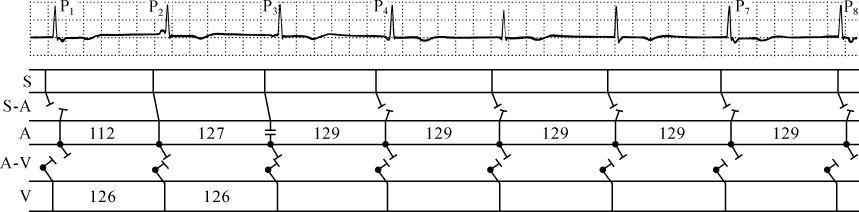
\includegraphics[width=5.80208in,height=1.42708in]{./images/Image00776.jpg}
 \captionsetup{justification=centering}
 \caption{例18 双重逸搏心律引起窦房、房室干扰性分离}
 \label{fig50-18}
  \end{figure} 

【心电图特征】

Ⅱ导联示P波形态有3种:①呈逆行P\textsuperscript{-}
波(如P\textsubscript{1} 、P\textsubscript{4} ~P\textsubscript{8}
),其P\textsuperscript{-} -P\textsuperscript{-}
间期规则,为1.29s,频率46次/min,逆行P\textsuperscript{-}
波重叠在QRS波群、ST段不同位置上;②直立P波(如P\textsubscript{2}
),为窦性P波;③呈浅倒P波(如P\textsubscript{3}
),形态介于窦性P波与逆行P\textsuperscript{-}
波之间,属房性融合波。P-R间期或R-P\textsuperscript{-}
间期长短不一,表明P波或P\textsuperscript{-}
波与QRS波群无关。QRS波形、时间正常,R-R间期规则,为1.26s,频率48次/min。ST段呈水平型延长达0.24s,T波倒置,Q-T间期0.53s(正常最高值为0.48s)。

【精解与讨论】

干扰性窦房分离是指窦性激动与起源于心房或能逆传心房的房室交接区、心室异位起搏点的激动在窦房交接区发生至少连续3次的绝对干扰现象。其发生机制系窦性与房性激动的频率相等或接近,或者能逆传心房的房室交接区、心室异位起搏点的频率略快于窦性,且前者激动抢先除极心房并逆传至窦房交接区与窦性冲动发生连续的绝对干扰所致。其心电图有以下特征:①有“纯”的窦性P波,即有明确的窦性P波;②有“纯”的房性异位P′波或逆行P\textsuperscript{-}
波;③在两个长的窦性P波或房性融合波间歇内至少出现3次P′波或P\textsuperscript{-}
波;④窦性P波的频率与房性异位P′波的频率相等或接近,或者逆行P\textsuperscript{-}
波的频率略快于窦性,但P-P间期与P′-P′(P\textsuperscript{-}
-P\textsuperscript{-}
)间期互差<0.09s;⑤长P-P间期与窦性基本周期呈倍数关系,至少呈4倍关系。干扰性窦房分离临床上比较少见。

本例P\textsubscript{2} 为窦性P波,P\textsubscript{3}
为房性融合波,其P\textsubscript{2} -P\textsubscript{3}
间期1.27s(频率47次/min)即为窦性基本周期,逆行P\textsuperscript{-}
波的P\textsuperscript{-} -P\textsuperscript{-}
间期规则,为1.29s,两者非常接近,虽然自P\textsubscript{3}
后未见窦性P波或者房性融合波出现,但根据P-P间期与P\textsuperscript{-}
-P\textsuperscript{-}
间期互差<0.09s,仍可诊断为不完全性干扰性窦房分离。因窦性频率虽然较心房下部逸搏心律或房室交接区上部(房-结区)逸搏心律的频率略快,但终因窦房结稍远离心房,其发放的冲动尚未传至心房,而心房下部或房室交接区上部(房-结区)异位起搏点却抢先激动心房并逆传,与窦性激动在窦房交接区发生连续干扰现象形成不完全性窦房分离。

本例逆行P\textsuperscript{-} 波的P\textsuperscript{-}
-P\textsuperscript{-}
间期规则,为1.29s,R-R间期亦规则,为1.26s,逆行P\textsuperscript{-}
波重叠在QRS波群、ST段不同位置上,表明P\textsuperscript{-}
波与QRS波群无关,系两个源异位起搏点发放冲动,P\textsuperscript{-}
波起源于心房下部或房室交接区上部(房-结区)的逸搏心律,QRS波群起源于房室交接区下部的逸搏心律,两者在房室交接区发生连续干扰而出现完全性房室分离。

干扰性窦房分离、房室分离本身是一种正常的生理性心电现象,其临床意义取决于上述两个起搏点的频率及基础心脏病的病因。若窦性频率持续<50次/min而出现下级起搏点被动发放,则提示窦房结功能低下,此时的房性逸搏或房室交接性逸搏具有避免心脏停跳的保护性代偿意义;若窦性频率正常而下级起搏点主动性地发放冲动,其频率61~130次/min,两者竞争性地控制心房,则为非阵发性房性心动过速或非阵发性房室交接性心动过速,多见于洋地黄中毒、急性心肌梗死、心肌炎、低钾血症及心脏手术等。

【心电图诊断】

①窦性心动过缓;②双重性逸搏心律(心房下部逸搏心律或房室交接区上部逸搏心律及其下部逸搏心律);③房性融合波;④不完全性干扰性窦房分离;⑤完全性干扰性房室分离;⑥Q-T间期延长以ST段水平型延长为主及T波改变,提示心肌供血不足。

例19 房室交接性逸搏伴不完全性反复搏动致自身节律被重整

【临床资料】

患者男性,36岁,临床诊断:病毒性心肌炎?

【心电图特征】

Ⅱ导联连续记录,窦性P-P间期0.76s,P-R间期0.13s,每隔2个窦性搏动延迟出现2个QRS-T波群,其QRS波群幅较窦性略高,其后有逆行P\textsuperscript{-}
波跟随,R-P\textsuperscript{-}
间期0.22s,逸搏周期为1.02s、1.32~1.40s短、长两种。ST段呈上斜型压低0.15~0.2mV。

\begin{figure}[!htbp]
 \centering
 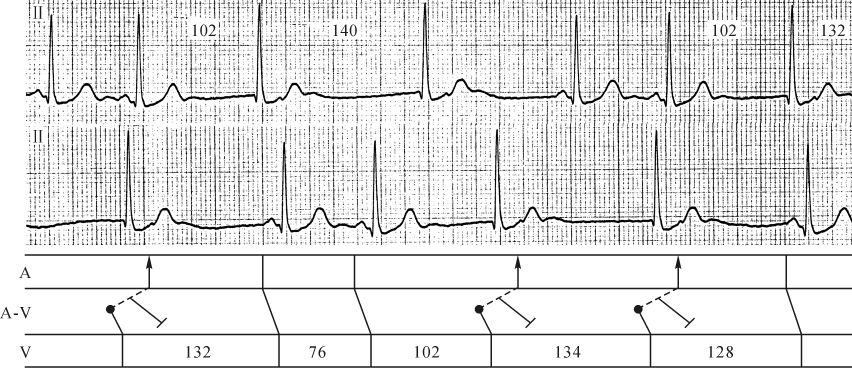
\includegraphics[width=5.76042in,height=2.48958in]{./images/Image00777.jpg}
 \captionsetup{justification=centering}
 \caption{例19 房室交接性逸搏伴不完全性反复搏动致自身节律被重整}
 \label{fig50-19}
  \end{figure} 

【精解与讨论】

本例窦性基本周期为0.76s,在R-R间期长达1.02s、1.32~1.40s时未见窦性P波出现,表明存在二度窦房传导阻滞或窦性停搏。单源性房室交接性逸搏周期一般是恒定的,本例逸搏周期为1.02s、1.32~1.40s短、长两种,提示本例房室交接性逸搏基本周期为1.02s,而长达1.32~1.40s
R-R间期,系其前房室交接性逸搏通过房室结慢径路逆传心房时又经快径路隐匿性地下传且重整了逸搏节律点所致,为房室交接性逸搏伴不完全性反复搏动致自身节律被重整。

【心电图诊断】

①成对的窦性搏动;②频发二度窦房传导阻滞或窦性停搏;③频发成对的房室交接性逸搏伴非时相性心室内差异性传导;④房室交接性逸搏伴不完全性反复搏动致自身节律被重整;⑤提示房室结内双径路传导;⑥ST段改变。

例20 房性早搏伴A型预激综合征及3相性右束支阻滞

【临床资料】

患者男性,20岁,反复发作心动过速5年,临床诊断:预激综合征、心肌炎?

【心电图特征】

Ⅱ导联示P波形态尖耸,电压0.25~0.30mV,P-R间期0.09s,有δ波,QRS波群时间0.12s;提早出现P′-QRS-T波群,其P′-R间期0.07s,有δ波,QRS波群明显增宽达0.16s;长V\textsubscript{1}
导联窦性搏动的P-R间期缩短,有δ波但没有Ⅱ导联明显,QRS波群时间0.12s,每隔1个窦性搏动提早出现1~2次P′-QRS-T波群,多数偶联间期由0.47s→0.36~0.38s缩短,下传的P′-R间期0.06~0.07s,δ波向上,第1个房性早搏的QRS波群明显增宽达0.16s,第2个房性早搏的QRS波群略窄为0.14s(梯形图A-V行中实线表示房室正道,虚线表示房室旁道、V行中斜影部分表示预激程度)。

【分析与讨论】

本例房性早搏多数呈成对出现,其P-P′间期、P′-P′间期由0.47s→0.36~0.38s缩短,提示房性早搏为折返性早搏,且在折返径路内传导速度逐渐加快,直至落在前一折返激动的绝对不应期而终止,出现折返径路内3:2反向文氏现象。房性早搏下传的P′-R间期较窦性的P-R间期缩短,犙犚犛波群时间较窦性QRS波群增宽,提示房性早搏均由旁道下传形成的完全性预激波形;第1个房性早搏QRS波群特别宽,主要是终末S波增宽,与其前长R-R间歇有关,即存在Ashman现象,系合并3相性右束支阻滞所致。

\begin{figure}[!htbp]
 \centering
 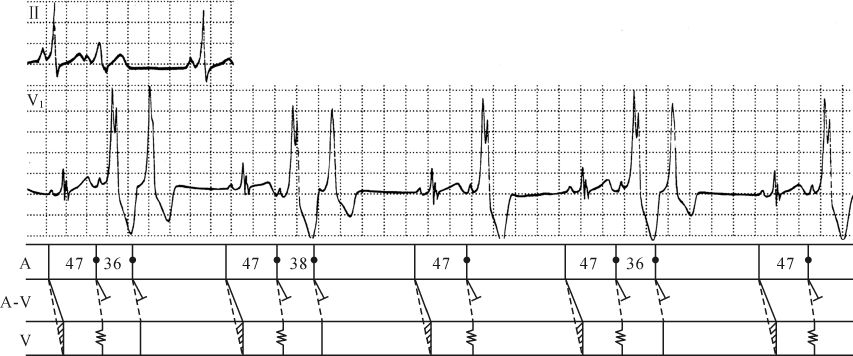
\includegraphics[width=5.76042in,height=2.40625in]{./images/Image00778.jpg}
 \captionsetup{justification=centering}
 \caption{例20 房性早搏伴A型预激综合征及3相性右束支阻滞}
 \label{fig50-20}
  \end{figure} 

预激综合征合并束支阻滞时,两者波形可同时并存或前者掩盖后者。当旁道终止部位远离束支阻滞所支配的部位,如A型预激合并右束支阻滞、B型预激合并左束支阻滞,则两者波形能同时显现;反之,当旁道终止部位恰好位于束支阻滞所支配的区域,如A型预激合并左束支阻滞、B型预激合并右束支阻滞,则预激波形将掩盖束支阻滞的波形。

【心电图诊断】

①窦性搏动;②肺型P波,不完全性右心房内传导阻滞?③A型预激综合征;④频发房性早搏伴完全性预激及3相性右束支阻滞,呈二、三联律;⑤心房折返径路内3:2反向文氏现象。

\protect\hypertarget{text00060.html}{}{}

\protect\hypertarget{text00060.htmlux5cux23chapter60}{}{}

